\documentclass[a4paper,12pt]{article}
\usepackage[utf8]{inputenc}
\usepackage[T1]{fontenc}
\usepackage[english]{babel}
\usepackage{color}
\usepackage{lmodern}
\usepackage{amsmath}
\usepackage{amssymb}
\usepackage{amsthm}
\usepackage{mathtools}
\usepackage[superscript]{cite}
\usepackage{listings}
\usepackage[ruled, linesnumbered, longend]{algorithm2e}
\usepackage{dsfont}
\usepackage{nicefrac}
\usepackage{upgreek}
\usepackage{paralist}
\usepackage{stmaryrd}
\usepackage{tikz}
\usepackage{pgffor}
\usepackage{pgfplots}
\usepackage{graphicx}
\usepackage{setspace}
\usepackage{fancyhdr}
% \usepackage[colorlinks=true,linkcolor=blue]{hyperref}				% Blue hyperlinks look better than red boxed ones

% Header
\newcommand\shorttitle{}
\newcommand\authors{Dominik Blank}

\fancyhf{} % sets all head and foot elements empty
\fancyhead[L]{\shorttitle}
\fancyhead[R]{\authors}
\fancyfoot[C]{\thepage}
\pagestyle{fancy} % sets the page style to the style delivered and editable with fancyhdr

% Own commands, operators, etc.
\newcommand{\abs}[1]{\lvert#1\rvert}
\newcommand{\norm}[1]{\lVert#1\rVert}

% Math environments
\theoremstyle{plain}
\newtheorem{theorem}{Theorem}[section]
\newtheorem{lemma}[theorem]{Lemma}
\newtheorem{corollary}[theorem]{Corollary}
\theoremstyle{definition}
\newtheorem{definition}[theorem]{Definition}
\theoremstyle{remark}
\newtheorem{remark}[theorem]{Remark}
\newtheorem{example}[theorem]{Example}

% END PREAMBLE

\author{Dominik Blank}
\title{On the influence of morphological operators on testing for a region of interest}

\onehalfspacing
\setlength{\parindent}{0pt}
\allowdisplaybreaks

\begin{document}
\begin{titlepage}

\newcommand{\HRule}{\rule{\linewidth}{0.5mm}} % Defines a new command for the horizontal lines, change thickness here

\center % Center everything on the page
 
%----------------------------------------------------------------------------------------
%	HEADING SECTIONS
%----------------------------------------------------------------------------------------

\textsc{\Large Georg-August-Universität Göttingen}\\[1.5cm] % Name of your university/college
%\textsc{\large }\\[0.5cm] % Major heading

%----------------------------------------------------------------------------------------
%	TITLE SECTION
%----------------------------------------------------------------------------------------

\HRule \\[0.4cm]
{\large \bfseries On the influence of morphological operators\\ on testing for a region of interest}\\[0.2cm] % Title of your document
\HRule \\[1cm]
\textsc{\large A thesis submitted for the degree of master of science in mathematics}\\[2cm] % Minor heading such as course title

%----------------------------------------------------------------------------------------
%	AUTHOR SECTION
%----------------------------------------------------------------------------------------

\begin{minipage}[t]{0.3\textwidth}
\begin{flushleft} \large
\emph{Author:}\\
Dominik \textsc{Blank}
\end{flushleft}
\end{minipage}
~
\begin{minipage}[t]{0.6\textwidth}
\begin{flushright} \large
\emph{Supervisors:} \\
Prof. Dr. Stephan \textsc{Huckemann}\\
Dr. Robin \textsc{Richter}
\end{flushright}
\end{minipage}\\[4cm]

%----------------------------------------------------------------------------------------
%	DATE SECTION
%----------------------------------------------------------------------------------------

{\large Göttingen, \today}\\[2cm] % Date, change the \today to a set date if you want to be precise

\begin{abstract}
	Morphological operations play an important role in fingerprint recognition. In this paper, we examine their effect on statistical significance in restricted statistical model.
\end{abstract}
\end{titlepage}

\newpage

\tableofcontents

\newpage

\section{Introduction}

\newpage

\section{Testing for a rectangular region of interest}

\subsection{Definitions}

\begin{definition}
	Let $M, N \in \mathbb{N}$ and $V \in \mathbb{R}^{M \times N}$ be a matrix. Assume there are two pairs of indices $(i_1, j_1), (i_2, j_2)$ with $1 \leq i_1 \leq i_2 \leq M$ and $1 \leq j_1 \leq j_2 \leq N$, such that
	\begin{equation}
		V(i, j) \neq 0 \textrm{ if and only if } (i, j) \in \{ i_1, \dots, i_2 \} \times \{ j_1, \dots, j_2 \}
	\end{equation}
	We call $R = \{ i_1, \dots, i_2 \} \times \{ j_1, \dots, j_2 \}$ a \emph{rectangular region of interest (rROI)} and say that $V$ contains the rROI $R$.
	
	Furthermore, we call $(i_1, j_1)$ the \emph{top left corner} and $(i_2, j_2)$ the \emph{bottom right corner} of $R$.
\end{definition}

\begin{definition}
	Let $M, N \in \mathbb{N}$ and $c \in \mathbb{R} \setminus \{ 0 \}$. Let $V \in \mathbb{R}^{M \times N}$ be a matrix, that only takes values in the set $\{ 0, \pm c \}$ and that contains a rectangular region of interest $R$. We say that $R$ has a \emph{checkerboard pattern}, if one of the following relations is true:
	\begin{subequations}
		\begin{align}
			\textrm{For all } (i, j) \in R: V(i, j) = c &\textrm{ if and only if } i + j \textrm{ is odd}.\\
			\textrm{For all } (i, j) \in R: V(i, j) = c &\textrm{ if and only if } i + j \textrm{ is even}.
		\end{align}
	\end{subequations}
\end{definition}

\begin{remark}
	If the first relation in the definition is true, that immediately implies, that
	\begin{equation*}
		\textrm{for all } (i, j) \in R: V(i, j) = - c \textrm{ if and only if } i + j \textrm{ is even},
	\end{equation*}
	since $V$ takes only values in $\{ 0, \pm c \}$, but for $(i, j) \in R$ we have $V(i,j) \neq 0$.
	Similarly, if the second relation is true, it implies that
	\begin{equation*}
		\textrm{for all } (i, j) \in R: V(i, j) = - c \textrm{ if and only if } i + j \textrm{ is odd}.
	\end{equation*}
	In both cases the values of $V$ alternate between $+c$ and $-c$ along the rows and columns of $R$. This is similar to the classical checkerboard pattern.
\end{remark}

\begin{definition}
	Let $M, N \in \mathbb{N}$ and $c \in \mathbb{R} \setminus \{ 0 \}$. We define $\mathcal{V}_c^{M, N}$ to be the set of all matrices $V \in \mathbb{R}^{M \times N}$, that only take values in the set $\{ 0, \pm c \}$ and that contain a rectangular region of interest with a checkerboard pattern.
\end{definition}

\newpage

\subsection{Statistical model}

Let $M, N \in \mathbb{N}$, $c \in \mathbb{R} \setminus \{ 0 \}$ and $G = \left\{ 1, \dots, M \right\} \times \left\{ 1, \dots, N \right\}$. Assume we are given noisy data
\begin{equation}\label{image}
	F(i, j) = c + V(i, j) + \varepsilon_{i, j}
\end{equation}
where $(i, j) \in G$, $V \in \mathcal{V}_c^{M, N}$ and $\varepsilon_{i, j} \sim \mathcal{N}(0, \sigma^2)$ are i.i.d. normal distributed random variables for some $\sigma > 0$ and for all $(i, j) \in G$.

Although defined as a matrix, we often refer to $F$ and $V$ as images and to $(i, j)$ as a pixel. Let $R$ be the rectangular region of interest contained in $V$. We aim to find a statistical test to determine for each individual pixel whether $(i, j) \in R$ or $(i, j) \notin R$.

To proceed we define for each pixel $(i, j) \in G$ the four values
\begin{align}
	D^\pm_1(i, j) &= V(i \pm 1, j) - V(i, j) \label{D1} \\
	D^\pm_2(i, j) &= V(i, j \pm 1) - V(i, j) \label{D2}
\end{align}
where we set
\begin{align*}
	V(i, 0) &= V(i, N) \\
	V(0, j) &= V(M, j) \\
	V(i, N+1) &= V(i, 1) \\
	V(M+1, j) &= V(1, j)
\end{align*}
to adjust to boundary issues. We now combine these values into two new values and assign to each pair $(i, j) \in G$ the values
\begin{equation}\label{D}
	D^\pm(i, j) = \sqrt{D_1^\pm(i, j)^2 + D_2^\pm(i, j)^2}
\end{equation}

Since we have assumed that $V \in \mathcal{V}_c^{M, N}$, we know that $V(i, j) = 0$ if and only if $(i, j) \notin R$. Let $(i_1, j_1)$ and $(i_2, j_2)$ be the top left and bottom right corner of $R$, respectively. Now, if $(i, j) \notin R$ it follows that $i \notin \{ i_1, \dots, i_2 \}$ or $j \notin \{ j_1, \dots, j_2 \}$. We have to distinguish four cases here:
\begin{align*}
	i < i_1 &\Rightarrow (i, j - 1) \notin R \textrm{ and } (i - 1, j) \notin R \\
	&\Rightarrow V(i, j - 1) = V(i - 1, j) = 0 \\
	j < j_1 &\Rightarrow (i - 1, j) \notin R \textrm{ and } (i, j - 1) \notin R \\
	&\Rightarrow V(i - 1, j) = V(i, j - 1) = 0 \\
	i > i_2 &\Rightarrow (i, j + 1) \notin R \textrm{ and } (i + 1, j) \notin R \\
	&\Rightarrow V(i, j + 1) = V(i + 1, j) = 0 \\
	j > j_2 &\Rightarrow (i + 1, j) \notin R \textrm{ and } (i, j + 1) \notin R \\
	&\Rightarrow V(i + 1, j) = V(i, j + 1) = 0
\end{align*}

We see, that in the first two cases, we have $D^-_1(i, j) = D^-_2(i, j) = 0$, which yields $D^-(i, j) = 0$. In the latter two cases, we get $D^+_1(i, j) = D^+_2(i, j) = 0$ and thus $D^+(i, j) = 0$. Thus, if $(i, j) \notin R$ it follows that $\min \{ D^+(i, j), D^-(i, j) \} = 0$.

On the other hand, we have assumed, that $R$ has a checkerboard pattern, thus $D^\pm(i, j) \neq 0$ for $(i, j) \in R$. This yields the equivalence
\begin{equation*}
	(i, j) \notin R \Leftrightarrow \min \{ D^+(i, j), D^-(i, j) \} = 0
\end{equation*}

Since our goal is to test for $(i, j) \in R$, we define a null hypothesis for each individual pixel:
\begin{equation}
	H_0(i, j): \min \{ D^+(i, j), D^-(i, j) \} = 0
\end{equation}

Unfortunately, we do not know the actual values of $V$, which makes $D^+$ and $D^-$ non-observable. We are given noisy data though. Based on the noisy data, we define four observable values for each pixel
\begin{align}
	\tilde{D}^\pm_1(i, j) &= F(i \pm 1, j) - F(i, j) \label{D1tilde} \\
	\tilde{D}^\pm_2(i, j) &= F(i, j \pm 1) - F(i, j) \label{D2tilde}
\end{align}
where we again define
\begin{align*}
	F(i, 0) &= F(i, N) \\
	F(0, j) &= F(M, j) \\
	F(i, N+1) &= F(i, 1) \\
	F(M+1, j) &= F(1, j)
\end{align*}
to adjust to boundary issues. Again we combine these values into two new values
\begin{equation}\label{Dtilde}
	\tilde{D}^\pm(i, j) = \sqrt{\tilde{D}_1^\pm(i, j)^2 + \tilde{D}_2^\pm(i, j)^2}
\end{equation}

We use these values for our test statistic and test for each individual pixel $(i, j)$ the null hypothesis
\begin{equation}
	H_0(i, j): \min \{ D^+(i, j), D^-(i, j) \} = 0
\end{equation}
against the alternative hypothesis
\begin{equation}
	H_1(i, j): \min \{ D^+(i, j), D^-(i, j) \} \neq 0
\end{equation}
using the test statistic
\begin{equation}
	T(i, j) = \min \{ \tilde{D}^+(i, j), \tilde{D}^-(i, j) \}
\end{equation}

\newpage

\subsection{Analysis of the statistical significance}

After having established our hypotheses and test statistic, we want to show, that we can ensure a given statistical significance $\alpha$. This will be done in two steps: The testing procedure is the combination of two testing procedures ($D^+$ and $D^-$) and we will see, that we can bound our combination by either of the individual ones. In a second step, we bound the individual procedures by computing their cumulative distribution function.

The first step is proven in the following lemma:
\begin{lemma}\label{lemtypeIbound}
	Assume the statistical model as above and let $D^\pm(i, j)$, $\tilde{D}^\pm(i, j)$, $T(i, j)$, $H_0(i, j)$ be defined as above. Then the following inequality holds:
	\begin{equation}\label{eqtypeIbound}
		\mathbb{P}(T(i, j) \geq t \mid H_0(i, j)) \leq \mathbb{P}(\tilde{D}^+(i, j) \geq t \mid D^+(i, j) = 0)
	\end{equation}
\end{lemma}
\begin{proof}
	If the null hypothesis for a given pixel $(i, j)$ is true, we can distinguish two cases: $D^+(i, j) = 0$ or $D^-(i, j) = 0$. Note, that these two cases are not exclusive. Without loss of generality we assume the case $D^+(i, j) = 0$. For $t \in \mathbb{R}^+$ we get the inequality
	\begin{align*}
		\mathbb{P}(T(i, j) \geq t \mid H_0(i, j)) &= \mathbb{P}(\min \{ \tilde{D}^+(i, j), \tilde{D}^-(i, j) \} \geq t \mid H_0(i, j)) \\
		&= \mathbb{P}(\{ \tilde{D}^+(i, j) \geq t \} \cap \{ \tilde{D}^-(i, j) \geq t \} \mid H_0(i, j)) \\
		&\leq \mathbb{P}(\tilde{D}^+(i, j) \geq t \mid H_0(i, j)) \\
		&= \mathbb{P}(\tilde{D}^+(i, j) \geq t \mid D^+(i, j) = 0)
	\end{align*}
	
	In the second case we get the same inequality by using the equality
	\begin{equation*}
		\mathbb{P}(\tilde{D}^-(i, j) \geq t \mid D^-(i, j) = 0) = \mathbb{P}(\tilde{D}^+(i, j) \geq t \mid D^+(i, j) = 0)
	\end{equation*}
\end{proof}

Equation \eqref{eqtypeIbound} shows that, if we can calculate the cumulative distribution function of $\tilde{D}^+(i, j)$ given $D^+(i, j) = 0$, we can bound the probability of a type I error in our testing procedure. The cumulative distribution function is given in the next theorem.
\begin{theorem}\label{thmeqcdf}
	Assume the statistical model as above and let $D^+(i, j)$ and $\tilde{D}^+(i, j)$ be defined as above. Then
	\begin{equation}\label{eqcdf}
		\begin{aligned}
			\mathbb{P}(\tilde{D}^+(i, j) \leq t \mid D^+(i, j) = 0) &= \frac{1}{\sqrt{3}} \left( \frac{3}{2} - \frac{3}{2} \exp \left( - \frac{t^2}{3 \sigma^2} \right) I_0 \left( \frac{t^2}{6 \sigma^2} \right) \right) - \sqrt{3} \\
			&\quad - \frac{2 - \sqrt{3}}{2} Q_1 \left( \frac{2 - \sqrt{3}}{6} \sqrt{\frac{t}{\sigma}}, \frac{2 + \sqrt{3}}{6} \sqrt{\frac{t}{\sigma}} \right) \\
			&\quad + \frac{2 + \sqrt{3}}{2} Q_1 \left( \frac{2 + \sqrt{3}}{6} \sqrt{\frac{t}{\sigma}}, \frac{2 - \sqrt{3}}{6} \sqrt{\frac{t}{\sigma}} \right)
		\end{aligned}
	\end{equation}
	where $I_0$ is the modified Bessel function of the first kind and $Q_M$ denotes the Marcum $Q$-function.
\end{theorem}
\begin{proof}
	In a first step, we note that by the definition of $D^+$ we get the equivalence
	\begin{equation*}
		D^+ = 0 \Leftrightarrow V(i + 1, j) - V(i, j) = V(i, j + 1) - V(i, j) = 0
	\end{equation*}
	
	Now we write out the left hand side of the equation, which we call $p(t)$, and use the equivalence above to get
	\begin{align*}
		p(t) &\coloneqq \mathbb{P}(\tilde{D}^+(i, j) \leq t \mid D^+(i, j) = 0) \\
		&= \mathbb{P}\big( (c + V(i + 1, j) + \varepsilon_{i + 1, j} - c - V(i, j) - \varepsilon_{i, j})^2 \\
		&\quad + (c + V(i, j + 1) + \varepsilon_{i, j + 1} - c - V(i, j) - \varepsilon_{i, j})^2 \leq t^2 \mid D^+(i, j) = 0 \big) \\
		&= \mathbb{P}\left( (\varepsilon_{i + 1, j} - \varepsilon_{i, j})^2 + (\varepsilon_{i, j + 1} - \varepsilon_{i, j})^2 \leq t^2 \right)
	\end{align*}
	
	Assuming the common term $\varepsilon_{i, j}$ to be constant and by defining
	\begin{align*}
		X_1 &= \varepsilon_{i + 1, j} - \varepsilon_{i, j} \sim \mathcal{N}(- \varepsilon_{i, j}, \sigma^2) \\
		X_2 &= \varepsilon_{i, j + 1} - \varepsilon_{i, j} \sim \mathcal{N}(- \varepsilon_{i, j}, \sigma^2)
	\end{align*}
	we obtain
	\begin{equation*}
		p(t) = \mathbb{P}\left( \sqrt{\left( \frac{X_1}{\sigma} \right)^2 + \left( \frac{X_2}{\sigma} \right)^2} \leq \frac{t}{\sigma} \right)
	\end{equation*}
	
	This shows, that the square root inside has a non-central Chi distribution with two degrees of freedom and non-centrality parameter
	\begin{equation*}
		\lambda = \sqrt{\left( \frac{- \varepsilon_{i, j}}{\sigma} \right)^2 + \left( \frac{- \varepsilon_{i, j}}{\sigma} \right)^2} = \frac{\sqrt{2} \abs{\varepsilon_{i, j}}}{\sigma}
	\end{equation*}
	and hence
	\begin{equation*}
		\sqrt{\left( \frac{X_1}{\sigma} \right)^2 + \left( \frac{X_2}{\sigma} \right)^2} \sim \chi_2 \left( \frac{\sqrt{2} \abs{\varepsilon_{i, j}}}{\sigma} \right)
	\end{equation*}
	
	Up until this point we assumed $\varepsilon_{i, j}$ to be constant, but it is a normal distributed random variable with zero mean and standard deviation $\sigma$. Thus, we have a compound probability distribution:
	\begin{align*}
		p(t) &= \mathbb{P}\left( \sqrt{\left( \frac{X_1}{\sigma} \right)^2 + \left( \frac{X_2}{\sigma} \right)^2} \leq \frac{t}{\sigma} \right) \\
		&= \int_0^\frac{t}{\sigma} \int_0^\infty \underbrace{x \exp \left( - \frac{x^2}{2} - \frac{\eta^2}{\sigma^2} \right) I_0 \left( \frac{\sqrt{2} \eta}{\sigma} x \right)}_{\textrm{pdf of} \ \chi_2 \left( \frac{\sqrt{2} \eta}{\sigma} \right) \ \textrm{for fixed} \ \eta} \underbrace{\frac{2}{\sqrt{2 \pi \sigma^2}} \exp \left( - \frac{\eta^2}{2 \sigma^2} \right)}_{\textrm{pdf of absolute value of} \ \mathcal{N}(0, \sigma^2)} \mathrm{d}\eta \mathrm{d}x \\
		&= \frac{2}{\sqrt{2 \pi \sigma^2}} \int_0^\frac{t}{\sigma} x \exp \left( - \frac{x^2}{2} \right) \int_0^\infty \exp \left( - \frac{3}{2 \sigma^2} \eta^2 \right) I_0 \left( \frac{\sqrt{2} x}{\sigma} \eta \right) \mathrm{d}\eta \mathrm{d}x
	\end{align*}
	
	where $I_0$ is the modified Bessel function of the first kind. We can solve the inner integral first. For $\mathrm{Re} \ \nu > -1$, $\mathrm{Re} \ \alpha > 0$ the following equality holds CITE!!!:
	\begin{equation}\label{eqintbessel}
		\int_0^\infty \exp \left( - \alpha x^2 \right) I_\nu ( \beta x ) \mathrm{d}x = \frac{\sqrt{\pi}}{2 \sqrt{\alpha}} \exp \left( \frac{\beta^2}{8 \alpha} \right) I_{\frac{1}{2} \nu} \left( \frac{\beta^2}{8 \alpha} \right)
	\end{equation}
	
	In our case, we have $\nu = 0$, $\alpha = \frac{3}{2 \sigma^2}$ and $\beta = \frac{\sqrt{2} x}{\sigma}$, which yields
	\begin{align*}
		\int_0^\infty \exp \left( - \frac{3}{2 \sigma^2} \eta^2 \right) I_0 \left( \frac{\sqrt{2} x}{\sigma} \eta \right) \mathrm{d}\eta &= \frac{\sqrt{\pi}}{2 \sqrt{\frac{3}{2 \sigma^2}}} \exp \left( \frac{\frac{2 x^2}{\sigma^2}}{8 \frac{3}{2 \sigma^2}} \right) I_0 \left( \frac{\frac{2 x^2}{\sigma^2}}{8 \frac{3}{2 \sigma^2}} \right) \\
		&= \frac{\sqrt{\pi} \sigma}{\sqrt{6}} \exp \left( \frac{x^2}{6} \right) I_0 \left( \frac{x^2}{6} \right)
	\end{align*}
	
	Plugging this in, we get
	\begin{align*}
		p(t) &= \frac{2}{\sqrt{2 \pi \sigma^2}} \int_0^\frac{t}{\sigma} x \exp \left( - \frac{x^2}{2} \right) \int_0^\infty \exp \left( - \frac{3}{2 \sigma^2} \eta^2 \right) I_0 \left( \frac{\sqrt{2} x}{\sigma} \eta \right) \mathrm{d}\eta \mathrm{d}x \\
		&= \frac{2}{\sqrt{2 \pi \sigma^2}} \int_0^\frac{t}{\sigma} x \exp \left( - \frac{x^2}{2} \right) \frac{\sqrt{\pi} \sigma}{\sqrt{6}} \exp \left( \frac{x^2}{6} \right) I_0 \left( \frac{x^2}{6} \right) \mathrm{d}x \\
		&= \frac{1}{\sqrt{3}} \int_0^\frac{t}{\sigma} x \exp \left( - \frac{x^2}{2} \right) \exp \left( \frac{x^2}{6} \right) I_0 \left( \frac{x^2}{6} \right) \mathrm{d}x \\
		&= \frac{1}{\sqrt{3}} \int_0^\frac{t}{\sigma} x \exp \left( - \frac{x^2}{3} \right) I_0 \left( \frac{x^2}{6} \right) \mathrm{d}x
	\end{align*}
	
	To proceed, we need to integrate by parts to replace the modified Bessel function $I_0$ with order zero by a modified Bessel function $I_1$ with order one.
	\begin{align*}
		p(t) &= \frac{1}{\sqrt{3}} \int_0^\frac{t}{\sigma} x \exp \left( - \frac{x^2}{3} \right) I_0 \left( \frac{x^2}{6} \right) \mathrm{d}x \\
		&= \frac{1}{\sqrt{3}} \left[ - \frac{3}{2} \exp \left( - \frac{x^2}{3} \right) I_0 \left( \frac{x^2}{6} \right) \right]_0^\frac{t}{\sigma} + \frac{1}{2 \sqrt{3}} \int_0^\frac{t}{\sigma} \exp \left( - \frac{x^2}{3} \right) x I_1 \left( \frac{x^2}{6} \right) \mathrm{d}x \\
		&= \frac{1}{\sqrt{3}} \left( \frac{3}{2} - \frac{3}{2} \exp \left( - \frac{t^2}{3 \sigma^2} \right) I_0 \left( \frac{t^2}{6 \sigma^2} \right) \right) + \frac{1}{2 \sqrt{3}} \int_0^\frac{t}{\sigma} \exp \left( - \frac{x^2}{3} \right) x I_1 \left( \frac{x^2}{6} \right) \mathrm{d}x
	\end{align*}
	
	In the next step we substitute $y = x^2$ in the remaining integral, which leaves us with
	\begin{equation*}
		p(t) = \frac{1}{\sqrt{3}} \left( \frac{3}{2} - \frac{3}{2} \exp \left( - \frac{t^2}{3 \sigma^2} \right) I_0 \left( \frac{t^2}{6 \sigma^2} \right) \right) + \frac{1}{4 \sqrt{3}} \int_0^\frac{t}{\sigma} \exp \left( - \frac{y}{3} \right) I_1 \left( \frac{y}{6} \right) \mathrm{d}y
	\end{equation*}
	
	We want to solve the remaining integral. Let $p \neq b$ and $s = \sqrt{p^2 - b^2}$, $u = \sqrt{a (p - s)}$ and $v = \sqrt{a (p + s)}$. Then CITE!!!
	\begin{equation}\label{eqintmarcum}
		\int_0^a \exp(-p x) I_M ( b x ) \mathrm{d}x = \frac{1}{s b^M} \left( (p - s)^M ( 1 - Q_M(u, v) ) - (p + s)^M ( 1 - Q_M(v, u) ) \right)
	\end{equation}
	where $Q_M$ denotes the Marcum $Q$-function. The Marcum $Q$-function is only defined for $M \geq 1$, which made the integration by parts necessary. Applying this equation with $M = 1$ to the integral yields
	\begin{align*}
		\int_0^\frac{t}{\sigma} \exp \left( - \frac{y}{3} \right) I_1 \left( \frac{y}{6} \right) \mathrm{d}y &= \frac{1}{\frac{1}{2 \sqrt{3}} \frac{1}{6}} \frac{2 - \sqrt{3}}{6} \left( 1 - Q_1 \left( \frac{2 - \sqrt{3}}{6} \sqrt{\frac{t}{\sigma}}, \frac{2 + \sqrt{3}}{6} \sqrt{\frac{t}{\sigma}} \right) \right) \\
		&\quad - \frac{1}{\frac{1}{2 \sqrt{3}} \frac{1}{6}} \frac{2 + \sqrt{3}}{6} \left( 1 - Q_1 \left( \frac{2 + \sqrt{3}}{6} \sqrt{\frac{t}{\sigma}}, \frac{2 - \sqrt{3}}{6} \sqrt{\frac{t}{\sigma}} \right) \right) \\
		&= 2 \sqrt{3} (2 - \sqrt{3}) \left( 1 - Q_1 \left( \frac{2 - \sqrt{3}}{6} \sqrt{\frac{t}{\sigma}}, \frac{2 + \sqrt{3}}{6} \sqrt{\frac{t}{\sigma}} \right) \right) \\
		&\quad - 2 \sqrt{3} (2 + \sqrt{3}) \left( 1 - Q_1 \left( \frac{2 + \sqrt{3}}{6} \sqrt{\frac{t}{\sigma}}, \frac{2 - \sqrt{3}}{6} \sqrt{\frac{t}{\sigma}} \right) \right)
	\end{align*}
	
	Plugging this in, we obtain the final result
	\begin{align*}
		p(t) &= \frac{1}{\sqrt{3}} \left( \frac{3}{2} - \frac{3}{2} \exp \left( - \frac{t^2}{3 \sigma^2} \right) I_0 \left( \frac{t^2}{6 \sigma^2} \right) \right) + \frac{1}{4 \sqrt{3}} \int_0^\frac{t}{\sigma} \exp \left( - \frac{y}{3} \right) I_1 \left( \frac{y}{6} \right) \mathrm{d}y \\
		&= \frac{1}{\sqrt{3}} \left( \frac{3}{2} - \frac{3}{2} \exp \left( - \frac{t^2}{3 \sigma^2} \right) I_0 \left( \frac{t^2}{6 \sigma^2} \right) \right) \\
		&\quad + \frac{2 \sqrt{3}}{4 \sqrt{3}} (2 - \sqrt{3}) \left( 1 - Q_1 \left( \frac{2 - \sqrt{3}}{6} \sqrt{\frac{t}{\sigma}}, \frac{2 + \sqrt{3}}{6} \sqrt{\frac{t}{\sigma}} \right) \right) \\
		&\quad - \frac{2 \sqrt{3}}{4 \sqrt{3}} (2 + \sqrt{3}) \left( 1 - Q_1 \left( \frac{2 + \sqrt{3}}{6} \sqrt{\frac{t}{\sigma}}, \frac{2 - \sqrt{3}}{6} \sqrt{\frac{t}{\sigma}} \right) \right) \\
		&= \frac{1}{\sqrt{3}} \left( \frac{3}{2} - \frac{3}{2} \exp \left( - \frac{t^2}{3 \sigma^2} \right) I_0 \left( \frac{t^2}{6 \sigma^2} \right) \right) - \sqrt{3} \\
		&\quad - \frac{2 - \sqrt{3}}{2} Q_1 \left( \frac{2 - \sqrt{3}}{6} \sqrt{\frac{t}{\sigma}}, \frac{2 + \sqrt{3}}{6} \sqrt{\frac{t}{\sigma}} \right) \\
		&\quad + \frac{2 + \sqrt{3}}{2} Q_1 \left( \frac{2 + \sqrt{3}}{6} \sqrt{\frac{t}{\sigma}}, \frac{2 - \sqrt{3}}{6} \sqrt{\frac{t}{\sigma}} \right)
	\end{align*}
\end{proof}

Thus, we have computed the distribution of $\tilde{D}(i, j)$ given $D^+(i, j) = 0$. Combining equations \eqref{eqtypeIbound} and \eqref{eqcdf} yields $\mathbb{P}(T(i, j) \geq t \mid H_0(i, j)) \leq 1 - p(t)$, where $p(t)$ is defined as in the proof of theorem \ref{thmeqcdf}. Let $\alpha \in (0, 1)$ be given. If we can find a threshold $t_\alpha$, such that $p(t_\alpha) \geq 1 - \alpha$, we have
\begin{equation}
	\mathbb{P}(T(i, j) \geq t_\alpha \mid H_0(i, j)) \leq 1 - p(t_\alpha) \leq \alpha
\end{equation}
and thus have assured a statistical significance of $\alpha$ in our testing procedure.

The easiest way to compute such a threshold would be to find the inverse function of $p(t)$. Since finding inverse functions of the modified Bessel function of the first kind $I_\nu$ and of the Marcum $Q$-function $Q_M$ is already complicated, there is unfortunately no easy way to compute an inverse function of $p(t)$. We can however compute a threshold $t_\alpha$ numerically. We will give a pseudocode here. A \emph{MATLAB} implementation of this pseudocode can be found in the appendix.\\

\begin{algorithm}[H]
	\KwIn{$\alpha \in (0, 1)$}
	\KwOut{$t_\alpha$ and $\alpha_{real}$, s.t. $p(t_\alpha) = 1 - \alpha_{real} \geq 1 - \alpha$}
	$t_\alpha = 0$\;
	$t_{inc} = 0.0001$\;
	\While{$p(t_\alpha) < 1 - \alpha$}
	{
		$t_\alpha + t_{inc}$\;
		$\alpha_{real} = 1 - p(t_\alpha)$\;
	}
	\caption{Computation of a threshold for a given statistical significance}
\end{algorithm}

\newpage

\subsection{Analysis of the power}

In equation \eqref{eqtypeIbound} we have managed to bound the probability of a type I error in our testing procedure by the probability of a type I error when testing for $D^+(i, j) = 0$ using the test statistic $\tilde{D}^+(i, j)$. We want to do the same for the probability of a type II error. The results are summarized in the following theorem.

\begin{theorem}\label{thmtypeIIbounds}
	Assume the statistical model as above and let $D^\pm(i, j)$, $\tilde{D}^\pm(i, j)$, $T(i, j)$, $H_1(i, j)$ be defined as above. Then the following inequalities hold:
	\begin{align}
		\mathbb{P}(T(i, j) \leq t \mid H_1(i, j)) &\leq 2 \cdot \mathbb{P}(\tilde{D}^+(i, j) \leq t \mid D^+(i, j) = \sqrt{2} c) \label{eqtypeIIupperbound} \\
		\mathbb{P}(T(i, j) \leq t \mid H_1(i, j)) &\geq \mathbb{P}(\tilde{D}^+(i, j) \leq t \mid D^+(i, j) = \sqrt{8} c) \label{eqtypeIIlowerbound}
	\end{align}
\end{theorem}
\begin{proof}
	Before we can prove the inequalities, we need some preparatory work: We have assumed, that $V$ only takes values in $\{ 0, \pm c \}$. This implies, that $D_1^+(i, j), D_2^+(i, j) \in \{ 0, \pm c, \pm 2 c \}$ and thus
	\begin{equation*}
		D^+(i, j) \in \{ 0, c, 2 c, \sqrt{2} c, \sqrt{5} c, \sqrt{8} c \}
	\end{equation*}
	
	We can narrow this list down even more. By assumption, $V$ contains a rectangular region of interest $R$ with a checkerboard pattern. This only allows the following combinations of $\abs{D_1^+(i, j)}$ and $\abs{D_2^+(i, j)}$:
	\begin{center}
		\begin{tabular}{c|c|c|c}
			\textbf{Position of pixels} $\mathbf{(i, j)}$, $\mathbf{(i + 1, j)}$, $\mathbf{(i, j + 1)}$ & $\mathbf{\abs{D_1^+(i, j)}}$ & $\mathbf{\abs{D_2^+(i, j)}}$ & $\mathbf{D^+(i, j)}$ \\
			\hline
			$(i, j), (i + 1, j), (i, j + 1) \notin R$ & $0$ & $0$ & $0$ \\
			\hline
			$(i, j), (i + 1, j) \notin R$ and $(i, j + 1) \in R$ & $0$ & $c$ & $c$ \\
			\hline
			$(i, j), (i, j + 1) \notin R$ and $(i + 1, j) \in R$ & $c$ & $0$ & $c$ \\
			\hline
			$(i, j) \in R$ and $(i + 1, j), (i, j + 1) \notin R$ & $c$ & $c$ & $\sqrt{2} c$ \\
			\hline
			$(i, j), (i + 1, j) \in R$ and $(i, j + 1) \notin R$ & $2 c$ & $c$ & $\sqrt{5} c$ \\
			\hline
			$(i, j), (i, j + 1) \in R$ and $(i + 1, j) \notin R$ & $c$ & $2 c$ & $\sqrt{5} c$ \\
			\hline
			$(i, j), (i + 1, j), (i, j + 1) \in R$ & $2 c$ & $2 c$ & $\sqrt{8} c$ \\
		\end{tabular}
	\end{center}
	
	It should be noted, that the case $(i, j) \in R$ and $(i + 1, j), (i, j + 1) \notin R$ can only happen at the bottom right corner of $R$.
	
	Other cases are not possible and thus $D^+(i, j) \in \{ 0, c, \sqrt{2} c, \sqrt{5} c, \sqrt{8} c \}$. We split this set of possible values into two sets. If $H_0(i, j) $ is true, then $(i, j) \notin R$ and thus $D^+(i, j) \in \{ 0, c \}$. On the other hand, if $H_1(i, j)$ is true, then $(i, j) \in R$ and thus $D^+(i, j) \in \{ \sqrt{2} c, \sqrt{5} c, \sqrt{8} c \}$. Based on this information we define the two sets $\mathcal{D}_0 = \{ 0, c \}$ and $\mathcal{D}_1 = \{ \sqrt{2} c, \sqrt{5} c, \sqrt{8} c \}$ and get the equivalences
	\begin{equation}
		\begin{aligned}
			H_0(i, j) &\Leftrightarrow D^+(i, j) \in \mathcal{D}_0 \\
			H_1(i, j) &\Leftrightarrow D^+(i, j) \in \mathcal{D}_1
		\end{aligned}
	\end{equation}
	
	Using this knowledge, we can find an upper bound for the probability of a type II error in our testing procedure:
	\begin{align*}
		\beta(t) &\coloneqq \mathbb{P}(T(i, j) \leq t \mid H_1(i, j)) \\
		&= \mathbb{P}(\min \{ \tilde{D}^+(i, j), \tilde{D}^-(i, j) \} \leq t \mid H_1(i, j)) \\
		&\leq \mathbb{P}(\tilde{D}^+(i, j) \leq t \mid H_1(i, j)) + \mathbb{P}(\tilde{D}^-(i, j) \leq t \mid H_1(i, j)) \\
		&= \mathbb{P}(\tilde{D}^+(i, j) \leq t \mid D^+(i, j) \in \mathcal{D}_1) + \mathbb{P}(\tilde{D}^-(i, j) \leq t \mid D^-(i, j) \in \mathcal{D}_1) \\
		&= 2 \cdot \mathbb{P}(\tilde{D}^+(i, j) \leq t \mid D^+(i, j) \in \mathcal{D}_1)
	\end{align*}
	where we used the equality
	\begin{equation*}
		\mathbb{P}(\tilde{D}^+(i, j) \leq t \mid D^+(i, j) \in \mathcal{D}_1) = \mathbb{P}(\tilde{D}^-(i, j) \leq t \mid D^-(i, j) \in \mathcal{D}_1)
	\end{equation*}
	in the last step. We can proceed by taking the specific $d \in \mathcal{D}_1$ that maximizes the probability. It is easy to see, that this is achieved, when $d$ is minimal and thus we get
	\begin{align*}
		\beta(t) &\leq 2 \cdot \mathbb{P}(\tilde{D}^+(i, j) \leq t \mid D^+(i, j) \in \mathcal{D}_1) \\
		&\leq 2 \cdot \max_{d \in \mathcal{D}_1} \mathbb{P}(\tilde{D}^+(i, j) \leq t \mid D^+(i, j) = d) \\
		&= 2 \cdot \mathbb{P}(\tilde{D}^+(i, j) \leq t \mid D^+(i, j) = \min_{d \in \mathcal{D}_1} d) \\
		&= 2 \cdot \mathbb{P}(\tilde{D}^+(i, j) \leq t \mid D^+(i, j) = \sqrt{2} c)
	\end{align*}
	which proves inequality \eqref{eqtypeIIupperbound}.
	
	Using similar techniques, we can also get a lower bound for the probability of a type II error:
	\begin{align*}
		\beta(t) &= \mathbb{P}(T(i, j) \leq t \mid H_1(i, j)) \\
		&= \mathbb{P}(\min \{ \tilde{D}^+(i, j), \tilde{D}^-(i, j) \} \leq t \mid H_1(i, j)) \\
		&\geq \mathbb{P}(\tilde{D}^+(i, j) \leq t \mid H_1(i, j)) \\
		&= \mathbb{P}(\tilde{D}^+(i, j) \leq t \mid D^+(i, j) \in \mathcal{D}_1)
	\end{align*}
	Again, we proceed by taking the specific $d \in \mathcal{D}_1$ that minimizes the probability. In this case, this is achieved, when $d$ is maximal. This yields
	\begin{align*}
		\beta(t) &\geq \mathbb{P}(\tilde{D}^+(i, j) \leq t \mid D^+(i, j) \in \mathcal{D}_1) \\
		&\geq \min_{d \in \mathcal{D}_1} \mathbb{P}(\tilde{D}^+(i, j) \leq t \mid D^+(i, j) = d) \\
		&= \mathbb{P}(\tilde{D}^+(i, j) \leq t \mid D^+(i, j) = \max_{d \in \mathcal{D}_1} d) \\
		&= \mathbb{P}(\tilde{D}^+(i, j) \leq t \mid D^+(i, j) = \sqrt{8} c)
	\end{align*}
	which proves inequality \eqref{eqtypeIIlowerbound} and finishes the proof.
\end{proof}

This result is the equivalent to lemma \ref{lemtypeIbound} for the probability of a type II error. We would like to find an equivalent result to theorem \ref{thmeqcdf} to write the bounds in the inequalities \eqref{eqtypeIIupperbound} and \eqref{eqtypeIIlowerbound} in terms of well-known functions like we did in equation \eqref{eqcdf}. Unfortunately, this would require more generalized versions of equalities \eqref{eqintbessel} and \eqref{eqintmarcum}.

We can however write down the compund probability distribution of the upper and lower bound as we did in the proof of theorem \ref{thmeqcdf}.

\begin{theorem}\label{thmcompprob}
	Assume the statistical model as above and let $D^+(i, j)$ and $\tilde{D}^+(i, j)$ be defined as above. Then the following equalities hold:
	\begin{equation}\label{eqcompprobupper}
		\begin{aligned}
			&\mathbb{P}(\tilde{D}^+(i, j) \leq t \mid D^+(i, j) = \sqrt{2} c) \\
			&= \frac{1}{\sqrt{2 \pi \sigma^2}} \int_0^\frac{t}{\sigma} x \exp \left( - \frac{x^2}{2} \right) \int_{-\infty}^\infty \exp \left( - \frac{(c - \eta)^2}{\sigma^2} - \frac{\eta^2}{2 \sigma^2} \right) I_0 \left( \frac{\sqrt{2} x}{\sigma} (c - \eta) \right) \mathrm{d}\eta \mathrm{d}x
		\end{aligned}
	\end{equation}
	\begin{equation}\label{eqcompproblower}
		\begin{aligned}
			&\mathbb{P}(\tilde{D}^+(i, j) \leq t \mid D^+(i, j) = \sqrt{8} c) \\
			&= \frac{1}{\sqrt{2 \pi \sigma^2}} \int_0^\frac{t}{\sigma} x \exp \left( - \frac{x^2}{2} \right) \int_{-\infty}^\infty \exp \left( - \frac{(2 c - \eta)^2}{\sigma^2} - \frac{\eta^2}{2 \sigma^2} \right) I_0 \left( \frac{\sqrt{2} x}{\sigma} (2 c - \eta) \right) \mathrm{d}\eta \mathrm{d}x
		\end{aligned}
	\end{equation}
\end{theorem}
\begin{proof}
	From the analysis of possible combinations of $D_1^+(i, j)$ and $D_2^+(i, j)$ in the proof of theorem \ref{thmtypeIIbounds} we can deduce the equivalences
	\begin{align*}
		\abs{D_1^+(i, j)} = \abs{D_2^+(i, j)} = c &\Leftrightarrow D^+(i, j) = \sqrt{2} c \\
		\abs{D_1^+(i, j)} = \abs{D_2^+(i, j)} = 2 c &\Leftrightarrow D^+(i, j) = \sqrt{8} c
	\end{align*}
	
	We proceed as in the proof of theorem \ref{thmeqcdf}. We have
	\begin{align*}
		&\mathbb{P}(\tilde{D}^+(i, j) \leq t \mid D^+(i, j) = \sqrt{2} c) \\
		&= \mathbb{P}\big( (c + V(i + 1, j) + \varepsilon_{i + 1, j} - c - V(i, j) - \varepsilon_{i, j})^2 \\
		&\quad + (c + V(i, j + 1) + \varepsilon_{i, j + 1} - c - V(i, j) - \varepsilon_{i, j})^2 \leq t^2 \mid D^+(i, j) = \sqrt{2} c \big) \\
		&= \mathbb{P}\left( (D_1^+ + \varepsilon_{i + 1, j} - \varepsilon_{i, j})^2 + (D_2^+ + \varepsilon_{i, j + 1} - \varepsilon_{i, j})^2 \leq t^2 \mid D^+(i, j) = \sqrt{2} c \right)
	\end{align*}
	
	We define the following random variables
	\begin{align*}
		\xi_1 &= D_1^+ - \varepsilon_{i, j} \sim \mathcal{N}(D_1^+, \sigma^2) \\
		\xi_2 &= D_2^+ - \varepsilon_{i, j} \sim \mathcal{N}(D_2^+, \sigma^2) \\
		X_1 &= \xi_1 + \varepsilon_{i + 1, j} \sim \mathcal{N}(\xi_1, \sigma^2) \\
		X_2 &= \xi_2 + \varepsilon_{i, j + 1} \sim \mathcal{N}(\xi_2, \sigma^2)
	\end{align*}
	and obtain
	\begin{align*}
		&\mathbb{P}(\tilde{D}^+(i, j) \leq t \mid D^+(i, j) = \sqrt{2} c) \\
		&= \mathbb{P}\left( \sqrt{\left( \frac{X_1}{\sigma} \right)^2 + \left( \frac{X_2}{\sigma} \right)^2} \leq \frac{t}{\sigma} \mid D^+(i, j) = \sqrt{2} c \right)
	\end{align*}
	
	Thus, we see, that the square root inside has a non-central Chi distribution with two degrees of freedom. The probability is conditioned on $D^+(i, j) = \sqrt{2} c$, which is equivalent to $\abs{D_1^+(i, j)} = \abs{D_2^+(i, j)} = c$. We can replace $\xi_1$ or $\xi_2$ by $- \xi_1$ or $- \xi_2$, respectively, without changing the probability. Thus, we can assume without loss of generality $D_1^+(i, j) = D_2^+(i, j) = c$. Assuming $\varepsilon_{i, j}$ to be constant, this non-central Chi distribution has non-centrality parameter
	\begin{equation*}
		\lambda = \sqrt{\left( \frac{D_1^+ - \varepsilon_{i, j}}{\sigma} \right)^2 + \left( \frac{D_2^+ - \varepsilon_{i, j}}{\sigma} \right)^2} = \frac{\sqrt{2} \abs{c - \varepsilon_{i, j}}}{\sigma}
	\end{equation*}
	
	This yields
	\begin{equation*}
		\sqrt{\left( \frac{X_1}{\sigma} \right)^2 + \left( \frac{X_2}{\sigma} \right)^2} \sim \chi_2 \left( \frac{\sqrt{2} \abs{c - \varepsilon_{i, j}}}{\sigma} \right)
	\end{equation*}
	
	Again, $\varepsilon_{i, j}$ is not constant, but a normal distributed random variable with zero mean and standard deviation $\sigma$. Thus, we have a compound probability distribution:
	\begin{align*}
		&\mathbb{P}(\tilde{D}^+(i, j) \leq t \mid D^+(i, j) = \sqrt{2} c) \\
		&= \mathbb{P}\left( \sqrt{\left( \frac{X_1}{\sigma} \right)^2 + \left( \frac{X_2}{\sigma} \right)^2} \leq \frac{t}{\sigma} \right) \\
		&= \int_0^\frac{t}{\sigma} \int_{-\infty}^\infty \underbrace{x \exp \left( - \frac{x^2}{2} - \frac{\abs{c - \eta}^2}{\sigma^2} \right) I_0 \left( \frac{\sqrt{2} \abs{c - \eta}}{\sigma} x \right)}_{\textrm{pdf of } \chi_2 \left( \frac{\sqrt{2} \abs{c - \eta}}{\sigma} \right) \textrm{ for fixed } \eta} \underbrace{\frac{1}{\sqrt{2 \pi \sigma^2}} \exp \left( - \frac{\eta^2}{2 \sigma^2} \right)}_{\textrm{pdf of } \mathcal{N}(0, \sigma^2)} \mathrm{d}\eta \mathrm{d}x \\
		&= \frac{1}{\sqrt{2 \pi \sigma^2}} \int_0^\frac{t}{\sigma} x \exp \left( - \frac{x^2}{2} \right) \int_{-\infty}^\infty \exp \left( - \frac{(c - \eta)^2}{\sigma^2} - \frac{\eta^2}{2 \sigma^2} \right) I_0 \left( \frac{\sqrt{2} x}{\sigma} (c - \eta) \right) \mathrm{d}\eta \mathrm{d}x
	\end{align*}
	where we used the symmetry of $I_0$. The second equality can be proven exactly the same way.
\end{proof}

While these results are not as strong as the result from theorem \ref{thmeqcdf}, they still give us two ways to estimate an upper and lower bound for the probability of a type II error in our testing procedure. Theorem \ref{thmtypeIIbounds} gives us the option to simulate the random variables and consequently the probabilities on the right hand side of equations \eqref{eqtypeIIupperbound} and \eqref{eqtypeIIlowerbound} to estimate an upper and lower bound. On the other hand, theorem \ref{thmcompprob} gives us the option to numerically integrate the right hand side of equations \eqref{eqcompprobupper} and \eqref{eqcompproblower} to get estimates of bounds for the probability of a type II error.

\newpage

\section{Binary morphological operations}

After having developed a basic testing procedure for extracting a rectangular region of interest, we now introduce morphological operations. It is our goal to study the influence of these operations on the statistical significance. Since we can view the output of the testing procedure as a binarization, it is sufficient to only consider \emph{binary} morphological operations. Moreover, we will only study the impact of \emph{binary opening} and \emph{binary closing}. These operations can be viewed as local, meaning they only depend on a limited and fixed number of pixels. In contrast to that, the \emph{convex hull} is a more global morphological operation depending on all pixels in an image, which makes it way harder to study on a pixel-by-pixel basis.

\subsection{Definition of opening \& closing}

Morphological binary opening and closing are closely related operations. They are both defined as a composition of \emph{binary erosion} and \emph{binary dilation}. Thus we start by defining those operations. It should be noted, that we focus on morphological operations in image processing and thus the definitions might differ from those in other contexts. All definitions are taken from CITE!!!.

\begin{definition}
	Let $A, B \subseteq \mathbb{Z}^n$.
	\begin{enumerate}
		\item The \emph{binary erosion} of $A$ by $B$ is defined as
		\begin{equation*}
			A \ominus B = \left\{ x \in \mathbb{Z}^n \mid x + b \in A \textrm{ for every } b \in B \right\}
		\end{equation*}
		\item The \emph{binary dilation} of $A$ by $B$ is defined as
		\begin{equation*}
			A \oplus B = \left\{ c \in \mathbb{Z}^n \mid c = a + b \textrm{ for some } a \in A \textrm{ and } b \in B \right\}
		\end{equation*}
	\end{enumerate}
	The set $B$ is called a \emph{structuring element}.
\end{definition}

\begin{remark}
	The set $B$ can be chosen arbitrarily, although should be chosen to fit the current application.
\end{remark}

As we can see, in binary morphology a binary image is a subset of $\mathbb{Z}^n$. This subset is the set of points at which the binary image is one. In contrast to that, we aim to study the influence of these morphological operations on the outcome of a statistical test for each individual pixel of an image. This outcome is best represented by a matrix $\varphi \in \{ 0, 1 \}^{M \times N}$. Hence, we need to translate the definition of binary opening and closing as operations on subsets of $\mathbb{Z}^n$ to operations on matrices $\varphi \in \{ 0, 1 \}^{M \times N}$. This gives rise to the following definition.

\begin{definition}
	Let $\varphi \in \{ 0, 1 \}^{M \times N}$. Let $B \subseteq \mathbb{Z}^2$ be a structuring element. We call
	\begin{equation*}
		A_\varphi \coloneqq \{ (i, j) \in \{ 1, \dots, M \} \times \{ 1, \dots, N \} \mid \varphi(i, j) = 1 \} \subseteq \mathbb{Z}^2
	\end{equation*}
	the \emph{index set of the binary matrix $\varphi$}.
	\begin{enumerate}
		\item The \emph{erosion of the binary matrix $\varphi$ by the structuring element $B$} is defined by
		\begin{equation}
			(\varphi \ominus B)(i, j) =
			\begin{cases}
				1, \textrm{ if } (i, j) \in A_\varphi \ominus B, \\
				0, \textrm{ if } (i, j) \notin A_\varphi \ominus B,
			\end{cases}
		\end{equation}
		for every $(i, j) \in \{ 1, \dots, M \} \times \{ 1, \dots, N \}$.
		\item The \emph{dilation of the binary matrix $\varphi$ by the structuring element $B$} is defined by
		\begin{equation}
			(\varphi \oplus B)(i, j) =
			\begin{cases}
				1, \textrm{ if } (i, j) \in A_\varphi \oplus B, \\
				0, \textrm{ if } (i, j) \notin A_\varphi \oplus B,
			\end{cases}
		\end{equation}
		for every $(i, j) \in \{ 1, \dots, M \} \times \{ 1, \dots, N \}$.
	\end{enumerate}
\end{definition}

By definition, erosion and dilation of a binary matrix are binary matrices as well, i.e. $\varphi \ominus B, \varphi \oplus B \in \{ 0, 1 \}^{M \times N}$.

We want to express $\varphi \ominus B$ and $\varphi \oplus B$ in terms of $\varphi$. This is done in the following lemma.

\begin{lemma}\label{lemerodil}
	Let $\varphi \in \{ 0, 1 \}^{M \times N}$ and $B \subseteq \mathbb{Z}^2$ be a structuring element. Let $(i, j) \in \{ 1, \dots, M \} \times \{ 1, \dots, N \}$. Then we have the following equalities:
	\begin{align}
		(\varphi \ominus B)(i, j) &= \prod_{(m, n) \in B} \varphi(i + m, j + n) \label{eqero} \\
		(\varphi \oplus B)(i, j) &= 1 - \prod_{(m, n) \in B} ( 1 - \varphi(i - m, j - n) ) \label{eqdil}
	\end{align}
	where we extend the matrix $\varphi$ to all of $\mathbb{Z}^2$ by setting $\varphi(k, l) = 0$ for $(k, l) \notin \{ 1, \dots, M \} \times \{ 1, \dots, N \}$.
\end{lemma}
\begin{proof}
	Let $A_\varphi$ be the index set of the binary matrix $\varphi$. We start with the first equality. By definition of binary erosion and using basic properties of set theory, we get the equivalence
	\begin{align*}
		(\varphi \ominus B)(i, j) = 1 &\Leftrightarrow (i, j) \in A_\varphi \ominus B \\
		&\Leftrightarrow \forall (m, n) \in B: (i, j) + (m, n) \in A_\varphi \\
		&\Leftrightarrow (i, j) \in \bigcap_{(m, n) \in B} ( A_\varphi - (m, n) )
	\end{align*}
	where we define the sets $A_\varphi - (m, n) \coloneqq \{ a - (m, n) \mid a \in A_\varphi \}$ for any $(m, n) \in \mathbb{Z}^2$.
	
	The sets $A_\varphi - (m, n)$ are related to the matrix $\varphi$ through the equivalence
	\begin{equation*}
		(i, j) \in ( A_\varphi - (m, n) ) \Leftrightarrow \varphi(i + m, j + n) = 1
	\end{equation*}
	
	Using this relation, we get the equivalence
	\begin{align*}
		(\varphi \ominus B)(i, j) = 1 &\Leftrightarrow (i, j) \in \bigcap_{(m, n) \in B} ( A_\varphi - (m, n) ) \\
		&\Leftrightarrow \prod_{(m, n) \in B} \varphi(i + m, j + n) = 1
	\end{align*}
	
	The functions on both sides of this equivalence only take values in $\{ 0, 1 \}$. Thus, we get a full equality
	\begin{equation*}
		(\varphi \ominus B)(i, j) = \prod_{(m, n) \in B} \varphi(i + m, j + n)
	\end{equation*}
	
	This proves the first equality.
	
	The proof of the second equality is quite similar. First we use the definition of binary dilation and basic set theory properties to get the equivalence
	\begin{align*}
		(\varphi \oplus B)(i, j) = 1 &\Leftrightarrow (i, j) \in A_\varphi \oplus B \\
		&\Leftrightarrow \exists (m, n) \in B: (i, j) - (m, n) \in A_\varphi \\
		&\Leftrightarrow (i, j) \in \bigcup_{(m, n) \in B} ( A_\varphi + (m, n) )
	\end{align*}
	
	The property $(i, j) \in \bigcup_{(m, n) \in B} ( A_\varphi + (m, n) )$ is fulfilled, if $\varphi(i - m, j - n) = 1$ for any $(m, n) \in B$. This observation yields the equivalence
	\begin{align*}
		(\varphi \oplus B)(i, j) = 1 &\Leftrightarrow (i, j) \in \bigcup_{(m, n) \in B} ( A_\varphi + (m, n) ) \\
		&\Leftrightarrow \prod_{(m, n) \in B} ( 1 - \varphi(i - m, j - n) ) = 0
	\end{align*}
	
	Since $\varphi$ is binary, $\prod_{(m, n) \in B} ( 1 - \varphi(i - m, j - n) )$ only takes values in $\{ 0, 1 \}$. Hence, we have the equivalence
	\begin{align*}
		(\varphi \oplus B)(i, j) = 1 &\Leftrightarrow \prod_{(m, n) \in B} ( 1 - \varphi(i - m, j - n) ) = 0 \\
		&\Leftrightarrow 1 - \prod_{(m, n) \in B} ( 1 - \varphi(i - m, j - n) ) = 1
	\end{align*}
	
	Again, since both sides are binary, this yields a full equality
	\begin{equation*}
		(\varphi \oplus B)(i, j) = 1 - \prod_{(m, n) \in B} ( 1 - \varphi(i - m, j - n) )
	\end{equation*}
\end{proof}

\begin{remark}
	The extension of $\varphi$ to all of $\mathbb{Z}^2$ is necessary, because in the product of the right hand side of equation \eqref{eqero} and \eqref{eqdil}, we might reach indices outside of $\{ 1, \dots, M \} \times \{ 1, \dots, N \}$.
\end{remark}

After having defined binary erosion and dilation, we now can define binary opening and closing. Again, we start by defining it for subsets of $\mathbb{Z}^n$ and then proceed to define it for binary matrices $\varphi \in \{ 0, 1 \}^{M \times N}$.
\begin{definition}
	Let $A, B \subseteq \mathbb{Z}^n$.
	\begin{enumerate}
		\item The \emph{binary opening} of $A$ by a structuring element $B$ is defined as
		\begin{equation*}
			A \circ B = (A \ominus B) \oplus B
		\end{equation*}
		\item The \emph{binary closing} of  $A$ by a structuring element $B$ is defined as
		\begin{equation*}
			A \bullet B = (A \oplus B) \ominus B
		\end{equation*}
	\end{enumerate}
\end{definition}

As we can see, binary opening and closing are concatenations of binary erosion and dilation. The definitions for matrices are done the same way, as they were done for erosion and dilation of binary matrices.

\begin{definition}
	Let $\varphi \in \{ 0, 1 \}^{M \times N}$, $B \subseteq \mathbb{Z}^2$ be a structuring element and $A_\varphi$ be the index set of $\varphi$.
	\begin{enumerate}
		\item The \emph{opening of the binary matrix $\varphi$ by the structuring element $B$} is defined by
		\begin{equation}
			(\varphi \circ B)(i, j) =
			\begin{cases}
				1, \textrm{ if } (i, j) \in A_\varphi \circ B, \\
				0, \textrm{ if } (i, j) \notin A_\varphi \circ B,
			\end{cases}
		\end{equation}
		for every $(i, j) \in \{ 1, \dots, M \} \times \{ 1, \dots, N \}$.
		\item The \emph{closing of the binary matrix $\varphi$ by the structuring element $B$} is defined by
		\begin{equation}
			(\varphi \bullet B)(i, j) =
			\begin{cases}
				1, \textrm{ if } (i, j) \in A_\varphi \bullet B, \\
				0, \textrm{ if } (i, j) \notin A_\varphi \bullet B,
			\end{cases}
		\end{equation}
		for every $(i, j) \in \{ 1, \dots, M \} \times \{ 1, \dots, N \}$.
	\end{enumerate}
\end{definition}

While we defined binary opening and closing for subsets of $\mathbb{Z}^2$ as concatenations of binary erosion and dilation, we did not define opening and closing of a binary matrix as concatenations of erosion and dilation of binary matrices. The following lemma shows the connection between these operations.

\begin{lemma}
	Let $\varphi \in \{ 0, 1 \}^{M \times N}$ and $B \subseteq \mathbb{Z}^2$ be a structuring element. We have the following connections between opening and closing and erosion and dilation of binary matrices:
	\begin{align}
		(\varphi \circ B) = (\varphi \ominus B) \oplus B \\
		(\varphi \bullet B) = (\varphi \oplus B) \ominus B
	\end{align}
\end{lemma}
\begin{proof}
	To prove these relations, we first show, that $A_{\varphi \ominus B} = A_\varphi \ominus B$ and $A_{\varphi \oplus B} = A_\varphi \oplus B$. By defintion of the index set of a binary matrix, we have
	\begin{align*}
		A_{\varphi \ominus B} &= \{ (i, j) \in \{ 1, \dots, M \} \times \{ 1, \dots, N \} \mid (\varphi \ominus B)(i, j) = 1 \} \\
		&= \{ (i, j) \in \{ 1, \dots, M \} \times \{ 1, \dots, N \} \mid (i, j) \in A_\varphi \ominus B \} \\
		&= A_\varphi \ominus B
	\end{align*}
	The second equality is proven similarly.
	
	Using this equality, we obtain
	\begin{align*}
		(\varphi \circ B)(i, j) = 1 &\Leftrightarrow (i, j) \in A_\varphi \circ B \\
		&\Leftrightarrow (i, j) \in (A_\varphi \ominus B) \oplus B \\
		&\Leftrightarrow (i, j) \in A_{\varphi \ominus B} \oplus B \\
		&\Leftrightarrow ((\varphi \ominus B) \oplus B)(i, j) = 1
	\end{align*}
	and thus prove the first relation.
	
	The proof of the second relation is analogous.
\end{proof}

After we established this connection, we can use the equalites deduced in lemma \ref{lemerodil} for erosion and dilation to derive similar equalities for opening and closing of a binary matrix.

\begin{corollary}
	Let $\varphi \in \{ 0, 1 \}^{M \times N}$ and $B \subseteq \mathbb{Z}^2$ be a structuring element. Let $(i, j) \in \{ 1, \dots, M \} \times \{ 1, \dots, N \}$. Then the following equalities hold:
	\begin{align}
		(\varphi \circ B)(i, j) &= 1 - \prod_{(m, n) \in B} \left( 1 - \left( \prod_{(\tilde{m}, \tilde{n}) \in B} \varphi(i - m + \tilde{m}, j - n + \tilde{n}) \right) \right) \label{eqopening} \\
		(\varphi \bullet B)(i, j) &= \prod_{(m, n) \in B} \left( 1 - \prod_{(\tilde{m}, \tilde{n}) \in B} ( 1 - \varphi(i + m - \tilde{m}, j + n - \tilde{n}) ) \right) \label{eqclosing}
	\end{align}
	where we extend the matrix $\varphi$ to all of $\mathbb{Z}^2$ by setting $\varphi(k, l) = 0$ for $(k, l) \notin \{ 1, \dots, M \} \times \{ 1, \dots, N \}$.
\end{corollary}
\begin{proof}
	We can use the previous lemma, as well as equation \eqref{eqdil} and finally equation \eqref{eqero} to obtain the first equality
	\begin{align*}
		(\varphi \circ B)(i, j) &= ((\varphi \ominus B) \oplus B)(i, j) \\
		&= 1 - \prod_{(m, n) \in B} ( 1 - (\varphi \ominus B)(i - m, j - n) ) \\
		&= 1 - \prod_{(m, n) \in B} \left( 1 - \left( \prod_{(\tilde{m}, \tilde{n}) \in B} \varphi(i - m + \tilde{m}, j - n + \tilde{n}) \right) \right)
	\end{align*}
	
	Using the same lemma and equations also yields the second equality
	\begin{align*}
		(\varphi \bullet B)(i, j) &= ((\varphi \oplus B) \ominus B)(i, j) \\
		&= \prod_{(m, n) \in B} (\varphi \oplus B)(i + m, j + n) \\
		&= \prod_{(m, n) \in B} \left( 1 - \prod_{(\tilde{m}, \tilde{n}) \in B} ( 1 - \varphi(i + m - \tilde{m}, j + n - \tilde{n}) ) \right)
	\end{align*}
	
	This finishes the proof.
\end{proof}

We now assume $\varphi(i, j)$ to be a random variable for all $(i, j) \in \{ 1, \dots, M \} \times \{ 1, \dots, N \}$. Equations \eqref{eqopening} and \eqref{eqclosing} show, that $(\varphi \circ B)(i, j)$ and $(\varphi \bullet B)(i, j)$ are random variables as well.

We want to express the events $\{ (\varphi \circ B)(i, j) = 1 \}$ and $\{ (\varphi \bullet B)(i, j) = 1 \}$ as unions and intersections of the events $\{ \varphi(i, j) = 1 \}$. This is done in the following corollary.

\begin{corollary}
	Let $M, N \in \mathbb{N}$ and $\varphi(i, j) \in \{ 0, 1 \}$ be a random variable for all $(i, j) \in \{ 1, \dots, M \} \times \{ 1, \dots, N \}$. Let $A$ be the index set of $\varphi$ and let $B \subseteq \mathbb{Z}^2$. Then we have the equivalences
	\begin{align}
		\{ (\varphi \circ B)(i, j) = 1 \} &\Leftrightarrow \bigcup_{(m, n) \in B} \bigcap_{(\tilde{m}, \tilde{n}) \in B} \{ \varphi(i - m + \tilde{m}, j - n + \tilde{n}) = 1 \} \label{eqeventopening} \\
		\{ (\varphi \bullet B)(i, j) = 1 \} &\Leftrightarrow \bigcap_{(m, n) \in B} \bigcup_{(\tilde{m}, \tilde{n}) \in B} \{ \varphi(i + m - \tilde{m}, j + n - \tilde{n}) = 1 \} \label{eqeventclosing}
	\end{align}
\end{corollary}
\begin{proof}
	Using equation \eqref{eqopening}, we obtain the equivalence
	\begin{align*}
		\{ (\varphi \circ B)(i, j) = 1 \} &\Leftrightarrow \left\{ 1 - \prod_{(m, n) \in B} \left( 1 - \left( \prod_{(\tilde{m}, \tilde{n}) \in B} \varphi(i - m + \tilde{m}, j - n + \tilde{n}) \right) \right) = 1 \right\} \\
		&\Leftrightarrow \left\{ \prod_{(m, n) \in B} \left( 1 - \left( \prod_{(\tilde{m}, \tilde{n}) \in B} \varphi(i - m + \tilde{m}, j - n + \tilde{n}) \right) \right) = 0 \right\}
	\end{align*}
	The event $\left\{ \prod_{(m, n) \in B} \left( 1 - \left( \prod_{(\tilde{m}, \tilde{n}) \in B} \varphi(i - m + \tilde{m}, j - n + \tilde{n}) \right) \right) = 0 \right\}$ occurs, if and only if any of the events $\left\{ 1 - \left( \prod_{(\tilde{m}, \tilde{n}) \in B} \varphi(i - m + \tilde{m}, j - n + \tilde{n}) \right) = 0 \right\}$ for $(m, n) \in B$ occurs. Thus, we get the equivalence
	\begin{align*}
		\{ (\varphi \circ B)(i, j) = 1 \} &\Leftrightarrow \left\{ \prod_{(m, n) \in B} \left( 1 - \left( \prod_{(\tilde{m}, \tilde{n}) \in B} \varphi(i - m + \tilde{m}, j - n + \tilde{n}) \right) \right) = 0 \right\} \\
		&\Leftrightarrow \bigcup_{(m, n) \in B} \left\{ 1 - \left( \prod_{(\tilde{m}, \tilde{n}) \in B} \varphi(i - m + \tilde{m}, j - n + \tilde{n}) \right) = 0 \right\} \\
		&\Leftrightarrow \bigcup_{(m, n) \in B} \left\{ \prod_{(\tilde{m}, \tilde{n}) \in B} \varphi(i - m + \tilde{m}, j - n + \tilde{n}) = 1 \right\}
	\end{align*}
	For fixed $(m, n) \in B$, the event $\left\{ \prod_{(\tilde{m}, \tilde{n}) \in B} \varphi(i - m + \tilde{m}, j - n + \tilde{n}) = 1 \right\}$ occurs, if and only if all of the events $\left\{ \varphi(i - m + \tilde{m}, j - n + \tilde{n}) = 1 \right\}$ for $(\tilde{m}, \tilde{n}) \in B$ occur. This yields the equivalence
	\begin{align*}
		\{ \varphi_{A \circ B}(i, j) = 1 \} &\Leftrightarrow \bigcup_{(m, n) \in B} \left\{ \prod_{(\tilde{m}, \tilde{n}) \in B} \varphi(i - m + \tilde{m}, j - n + \tilde{n}) = 1 \right\} \\
		&\Leftrightarrow \bigcup_{(m, n) \in B} \bigcap_{(\tilde{m}, \tilde{n}) \in B} \{ \varphi(i - m + \tilde{m}, j - n + \tilde{n}) = 1 \}
	\end{align*}
	
	This finishes the proof of first equivalence. The proof of the second equivalence is analogous.
\end{proof}

\newpage

\subsection{Examples}

\newpage

\section{Main results}

\begin{theorem}
	Assume the following statistical model:
	
	Let $M, N \in \mathbb{N}$ and $G = \left\{ 1, \dots, M \right\} \times  \left\{ 1, \dots, N \right\}$. We are given data
	\begin{equation}\label{f}
		F(i, j) = c + V(i, j) + \varepsilon_{i, j}
	\end{equation}
	where $(i, j) \in G$, $c \in \mathbb{R}$ is constant, $V \in \mathcal{V}_c^{M, N}$ and $\varepsilon_{i, j} \sim \mathcal{N}(0, \sigma^2)$ are i.i.d. normal distributed random variables for some $\sigma > 0$ and for all $(i, j) \in G$.
	
	Let $T(i, j)$ denote the testing procedure developed in the previous sections. Let $\alpha \in (0, 1)$ and $t_\alpha$ be the threshold to ensure a statistical significance of $\alpha$ in the testing procedure. Let $\varphi_\alpha$ be the binary image defined by
	\begin{equation}
		\varphi_\alpha(i, j) = \mathds{1}_{ \{ T(i, j) \geq t_\alpha \} }
	\end{equation}
	for all $(i, j) \in G$ and let $A_\alpha \coloneqq A_{\varphi_\alpha}$ be the index set of $\varphi_\alpha$.
	
	Let $k \in \mathbb{N}$ be odd. Let $K = \{ -\frac{k - 1}{2}, -\frac{k - 3}{2}, \dots, \frac{k - 3}{2}, \frac{k - 1}{2} \}$ and $B = K \times K$ be a structuring element.
	Then the following inequalities hold:
	\begin{align}
		\mathbb{P}((\varphi_\alpha \circ B)(i, j) = 1 \mid H_0(i, j)) \leq k \alpha^{\frac{k+1}{2}} \label{ineqopening} \\
		\mathbb{P}((\varphi_\alpha \bullet B)(i, j) = 1 \mid H_0(i, j)) \leq k^2 \alpha \label{ineqclosing}
	\end{align}
\end{theorem}
\begin{proof}
	We start with the proof of inequality \eqref{ineqopening}. We aim to find an upper bound for the probability
	\begin{equation*}
		\mathbb{P}((\varphi_\alpha \circ B)(i, j) = 1 \mid H_0(i, j))
	\end{equation*}
	
	Let $(i_1, j_1)$ be the top right corner and $(i_2, j_2)$ the bottom right corner of the rectangular region of interest contained in $V$. We first notice that $H_0(i, j)$ is equivalent to $V(i, j) = 0$. Since $V$ contains a rectangular region of interest, this means that $i < i_1$ or $i > i_2$ or $j < j_1$ or $j > j_2$. We need to differentiate cases here. These four cases are not mutually exclusive, but have different implications for the row/column of the index $(i, j)$ and a neighbouring row/column:\\
	
	\begin{tabular}{|c|c|c|}
		\hline
		\textbf{case} & \textbf{row/column of $(i, j)$} & \textbf{neighbouring row/column} \\
		\hline
		$i < i_1$ & $V(i, 1) = \dots = V(i, N) = 0$ & $V(i-1, 1) = \dots = V(i-1, N) = 0$ \\
		\hline
		$i > i_2$ & $V(i, 1) = \dots = V(i, N) = 0$ & $V(i+1, 1) = \dots = V(i+1, N) = 0$ \\
		\hline
		$j < j_1$ & $V(1, j) = \dots = V(M, j) = 0$ & $V(1, j-1) = \dots = V(M, j-1) = 0$ \\
		\hline
		$j > j_2$ & $V(1, j) = \dots = V(M, j) = 0$ & $V(1, j+1) = \dots = V(M, j+1) = 0$ \\
		\hline
	\end{tabular}\\
	
	Without loss of generality we assume the first case. This implies that
	\begin{equation*}
		D^-(i, 1) = \dots = D^-(i, N) = 0
	\end{equation*}
	
	In a first step, we use equivalence \eqref{eqeventopening} and the fact, that $B = K \times K$ to write this probability as
	\begin{align*}
		\mathbb{P}&( (\varphi_\alpha \circ B)(i, j) = 1 \mid H_0(i, j) ) \\
		&= \mathbb{P}\left( \bigcup_{(m, n) \in B} \bigcap_{(\tilde{m}, \tilde{n}) \in B} \{ \varphi_\alpha(i - m + \tilde{m}, j - n + \tilde{n}) = 1 \} \mid H_0(i, j) \right) \\
		&= \mathbb{P}\left( \bigcup_{m, n \in K} \bigcap_{\tilde{m}, \tilde{n} \in K} \{ \varphi_\alpha(i - m + \tilde{m}, j - n + \tilde{n}) = 1 \} \mid H_0(i, j) \right)
	\end{align*}
	
	We now want to bound this from above by writing it as a sum over $n \in K$ and get
	\begin{align*}
		\mathbb{P}&( (\varphi_\alpha \circ B)(i, j) = 1 \mid H_0(i, j) ) \\
		&= \mathbb{P}\left( \bigcup_{m, n \in K} \bigcap_{\tilde{m}, \tilde{n} \in K} \{ \varphi_\alpha(i - m + \tilde{m}, j - n + \tilde{n}) = 1 \} \mid H_0(i, j) \right) \\
		&\leq \sum_{n \in K} \mathbb{P}\left( \bigcup_{m \in K} \bigcap_{\tilde{m}, \tilde{n} \in K} \{ \varphi_\alpha(i - m + \tilde{m}, j - n + \tilde{n}) = 1 \} \mid H_0(i, j) \right)
	\end{align*}
	
	By dropping every term except for $\tilde{m} = m$ in the intersection inside, we get the upper bound
	\begin{align*}
		\mathbb{P}&( (\varphi_\alpha \circ B)(i, j) = 1 \mid H_0(i, j) ) \\
		&\leq \sum_{n \in K} \mathbb{P}\left( \bigcup_{m \in K} \bigcap_{\tilde{m}, \tilde{n} \in K} \{ \varphi_\alpha(i - m + \tilde{m}, j - n + \tilde{n}) = 1 \} \mid H_0(i, j) \right) \\
		&\leq \sum_{n \in K} \mathbb{P}\left( \bigcup_{m \in K} \bigcap_{\tilde{m} = m, \tilde{n} \in K} \{ \varphi_\alpha(i - m + \tilde{m}, j - n + \tilde{n}) = 1 \} \mid H_0(i, j) \right) \\
		&= \sum_{n \in K} \mathbb{P}\left( \bigcup_{m \in K} \bigcap_{\tilde{n} \in K} \{ \varphi_\alpha(i, j - n + \tilde{n}) = 1 \} \mid H_0(i, j) \right)
	\end{align*}
	
	The events inside the probability do not depend on $m \in K$ anymore, which yields
	\begin{equation*}
		\bigcup_{m \in K} \bigcap_{\tilde{n} \in K} \{ \varphi_\alpha(i, j - n + \tilde{n}) = 1 \} = \bigcap_{\tilde{n} \in K} \{ \varphi_\alpha(i, j - n + \tilde{n}) = 1 \}
	\end{equation*}
	
	By plugging this in, we obtain the upper bound
	\begin{align*}
		\mathbb{P}&( (\varphi_\alpha \circ B)(i, j) = 1 \mid H_0(i, j) ) \\
		&\leq \sum_{n \in K} \mathbb{P}\left( \bigcup_{m \in K} \bigcap_{\tilde{n} \in K} \{ \varphi_\alpha(i, j - n + \tilde{n}) = 1 \} \mid H_0(i, j) \right) \\
		&= \sum_{n \in K} \mathbb{P}\left( \bigcap_{\tilde{n} \in K} \{ \varphi_\alpha(i, j - n + \tilde{n}) = 1 \} \mid H_0(i, j) \right)
	\end{align*}
	
	We have defined the binary $\varphi_\alpha$ by setting $\varphi_\alpha(i, j) = \mathds{1}_{ \{ T(i, j) \geq t_\alpha \} }$. Using this definition and the definition of $T(i, j)$ we can rewrite the upper bound as
	\begin{align*}
		&\sum_{n \in K} \mathbb{P}\left( \bigcap_{\tilde{n} \in K} \{ \varphi_\alpha(i, j - n + \tilde{n}) = 1 \} \mid H_0(i, j) \right) \\
		&= \sum_{n \in K} \mathbb{P}\left( \bigcap_{\tilde{n} \in K} \{ T(i, j - n + \tilde{n}) \geq t_\alpha \} \mid H_0(i, j) \right) \\
		&= \sum_{n \in K} \mathbb{P}\left( \bigcap_{\tilde{n} \in K} \left( \{ \tilde{D}^+(i, j - n + \tilde{n}) \geq t_\alpha \} \cap \{ \tilde{D}^-(i, j - n + \tilde{n}) \geq t_\alpha \} \right) \mid H_0(i, j) \right)
	\end{align*}
	
	By dropping the events $\{ \tilde{D}^+(i, j - n + \tilde{n}) \geq t_\alpha \}$, we get
	\begin{align*}
		\mathbb{P}&( (\varphi_\alpha \circ B)(i, j) = 1 \mid H_0(i, j) ) \\
		&\leq \sum_{n \in K} \mathbb{P}\left( \bigcap_{\tilde{n} \in K} \left( \{ \tilde{D}^+(i, j - n + \tilde{n}) \geq t_\alpha \} \cap \{ \tilde{D}^-(i, j - n + \tilde{n}) \geq t_\alpha \} \right) \mid H_0(i, j) \right) \\
		&\leq \sum_{n \in K} \mathbb{P}\left( \bigcap_{\tilde{n} \in K} \{ \tilde{D}^-(i, j - n + \tilde{n}) \geq t_\alpha \} \mid H_0(i, j) \right)
	\end{align*}
	
	We now define a second set $K_1 = \{ -\frac{k - 1}{2}, -\frac{k - 5}{2}, \dots, \frac{k - 5}{2}, \frac{k - 1}{2} \}$. We have $K_1 \subseteq K$. Since $\tilde{D}^-(i, j)$ only depends on the pixels $(i, j), (i - 1, j), (i, j - 1)$, we see, that for fixed $n \in K$ the set $\{ \tilde{D}^-(i, j - n + \tilde{n}) \mid \tilde{n} \in K_1 \}$ is a set of independent random variables. We drop the terms in $K \setminus K_1$ and use the independence to obtain
	\begin{align*}
		\mathbb{P}&( (\varphi_\alpha \circ B)(i, j) = 1 \mid H_0(i, j) ) \\
		&\leq \sum_{n \in K} \mathbb{P}\left( \bigcap_{\tilde{n} \in K} \{ \tilde{D}^-(i, j - n + \tilde{n}) \geq t_\alpha \} \mid H_0(i, j) \right) \\
		&\leq \sum_{n \in K} \mathbb{P}\left( \bigcap_{\tilde{n} \in K_1} \{ \tilde{D}^-(i, j - n + \tilde{n}) \geq t_\alpha \} \mid H_0(i, j) \right) \\
		&= \sum_{n \in K} \prod_{\tilde{n} \in K_1} \mathbb{P}\left( \tilde{D}^-(i, j - n + \tilde{n}) \geq t_\alpha \mid H_0(i, j) \right)
	\end{align*}
	
	At the start of this proof, we have observed that $H_0(i, j)$ implies one of the four cases listed in the table above. On the other hand, any of the cases implies $H_0(i, j)$. This equivalence is obtained through the prior knowledge, that $V$ contains a rectangular region of interest. We have assumed the first case and thus get
	\begin{align*}
		\mathbb{P}&( (\varphi_\alpha \circ B)(i, j) = 1 \mid H_0(i, j) ) \\
		&\leq \sum_{n \in K} \prod_{\tilde{n} \in K_1} \mathbb{P}\left( \tilde{D}^-(i, j - n + \tilde{n}) \geq t_\alpha \mid H_0(i, j) \right) \\
		&= \sum_{n \in K} \prod_{\tilde{n} \in K_1} \mathbb{P}\left( \tilde{D}^-(i, j - n + \tilde{n}) \geq t_\alpha \mid D^-(i, 1) = \dots = D^-(i, N) = 0 \right) \\
		&= \sum_{n \in K} \prod_{\tilde{n} \in K_1} \mathbb{P}\left( \tilde{D}^-(i, j - n + \tilde{n}) \geq t_\alpha \mid D^-(i, j - n + \tilde{n}) = 0 \right)
	\end{align*}
	
	By assumption, $t_\alpha$, such that a statistical significance of $\alpha$ was assured in the testing procedure. This is done by using lemma \ref{lemtypeIbound} and theorem \ref{thmeqcdf} by bounding the probability $\mathbb{P}(\tilde{D}^+(i, j) \geq t \mid D^+(i, j) = 0)$ by $\alpha$. This yields
	\begin{align*}
		\mathbb{P}&( (\varphi_\alpha \circ B)(i, j) = 1 \mid H_0(i, j) ) \\
		&\leq \sum_{n \in K} \prod_{\tilde{n} \in K_1} \mathbb{P}\left( \tilde{D}^-(i, j - n + \tilde{n}) \geq t_\alpha \mid D^-(i, j - n + \tilde{n}) = 0 \right) \\
		&\leq \sum_{n \in K} \prod_{\tilde{n} \in K_1} \alpha \\
		&= \abs{K} \alpha^{\abs{K_1}} \\
		&= k \alpha^{\frac{k+1}{2}}
	\end{align*}
	
	This proves the first inequality for the first case. The other three cases can be proven analogously by swapping the roles of $m$ or $\tilde{m}$ with $n$ or $\tilde{n}$, respectively and/or by replacing $D^-$ by $D^+$. This finishes the proof of the first inequality.\\
	
	
	For the proof of the second inequality, we want to exploit our prior knowledge on $V$ again. As already stated in the proof of the first inequlity, we see, that $H_0(i, j)$ is equivalent to $V(i, j) = 0$, which is equivalent to at least one of the cases $i < i_1$ or $i > i_2$ or $j < j_1$ or $j > j_2$ being true.
	
	By differentiating cases, we can observe implications for other rows or columns of $V$ depending on the case:\\
	
	\begin{tabular}{|c|c|}
		\hline
		\textbf{case} & \textbf{other rows/columns of $V$} \\
		\hline
		$i < i_1$ & $\forall r \in \{ 1, \dots, i \}: V(r, 1) = \dots = V(r, N) = 0$ \\
		\hline
		$i > i_2$ & $\forall r \in \{ i, \dots, M \}: V(r, 1) = \dots = V(r, N) = 0$ \\
		\hline
		$j < j_1$ & $\forall s \in \{ 1, \dots, j \}: V(1, s) = \dots = V(M, s) = 0$ \\
		\hline
		$j > j_2$ & $\forall s \in \{ j, \dots, N \}: V(1, s) = \dots = V(M, s) = 0$ \\
		\hline
	\end{tabular}\\
	
	Without loss of generality we assume the first case. This implies that
	\begin{equation*}
		\forall r \in \{ 1, \dots, i \}: D^-(r, 1) = \dots = D^-(r, N) = 0
	\end{equation*}
	and thus, that the null hypotheses $H_0(r, 1), \dots, H_0(r, N)$ are true for all $r \in \{ 1, \dots, i \}$.
	
	Set $m_0 = -\frac{k - 1}{2}$ and $n_0 = 0$. Then $(m_0, n_0) \in B$ and we get that the null hypotheses $H_0(i + m_0 - \tilde{m}, j + n_0 - \tilde{n})$ are true for all $\tilde{m}, \tilde{n} \in K$. Moreover, we have $D^-(i + m_0 - \tilde{m}, j + n_0 - \tilde{n}) = 0$ for all $\tilde{m}, \tilde{n} \in K$.
	
	We use equivalence \eqref{eqeventclosing} and $B = K \times K$ to write the left hand side of inequality \eqref{ineqclosing} as
	\begin{align*}
		\mathbb{P}&( (\varphi_\alpha \bullet B)(i, j) = 1 \mid H_0(i, j) ) \\
		&= \mathbb{P}\left( \bigcap_{(m, n) \in B} \bigcup_{(\tilde{m}, \tilde{n}) \in B} \{ \varphi_\alpha(i + m - \tilde{m}, j + n - \tilde{n}) = 1 \} \mid H_0(i, j) \right) \\
		&= \mathbb{P}\left( \bigcap_{m, n \in K} \bigcup_{\tilde{m}, \tilde{n} \in K} \{ \varphi_\alpha(i + m - \tilde{m}, j + n - \tilde{n}) = 1 \} \mid H_0(i, j) \right)
	\end{align*}
	
	By dropping every term in the intersection except for $m = m_0$ and $n = n_0$ we can bound this from above
	\begin{align*}
		\mathbb{P}&( (\varphi_\alpha \bullet B)(i, j) = 1 \mid H_0(i, j) ) \\
		&= \mathbb{P}\left( \bigcap_{m, n \in K} \bigcup_{\tilde{m}, \tilde{n} \in K} \{ \varphi_\alpha(i + m - \tilde{m}, j + n - \tilde{n}) = 1 \} \mid H_0(i, j) \right) \\
		&\leq \mathbb{P}\left( \bigcup_{\tilde{m}, \tilde{n} \in K} \{ \varphi_\alpha(i + m_0 - \tilde{m}, j + n_0 - \tilde{n}) = 1 \} \mid H_0(i, j) \right) \\
		&= \mathbb{P}\left( \bigcup_{\tilde{m}, \tilde{n} \in K} \{ \varphi_\alpha(i + m_0 - \tilde{m}, j - \tilde{n}) = 1 \} \mid H_0(i, j) \right)
	\end{align*}
	
	Writing this as the sum over all $\tilde{m}, \tilde{n} \in K$ yields
	\begin{align*}
		\mathbb{P}&( (\varphi_\alpha \bullet B)(i, j) = 1 \mid H_0(i, j) ) \\
		&\leq \mathbb{P}\left( \bigcup_{\tilde{m}, \tilde{n} \in K} \{ \varphi_\alpha(i + m_0 - \tilde{m}, j - \tilde{n}) = 1 \} \mid H_0(i, j) \right) \\
		&\leq \sum_{\tilde{m}, \tilde{n} \in K} \mathbb{P}\left( \varphi_\alpha(i + m_0 - \tilde{m}, j - \tilde{n}) = 1 \mid H_0(i, j) \right)
	\end{align*}
	
	By definition of $\varphi_\alpha$ and $T$ this can be written as
	\begin{align*}
		\mathbb{P}&( (\varphi_\alpha \bullet B)(i, j) = 1 \mid H_0(i, j) ) \\
		&\leq \sum_{\tilde{m}, \tilde{n} \in K} \mathbb{P}\left( \varphi_\alpha(i + m_0 - \tilde{m}, j - \tilde{n}) = 1 \mid H_0(i, j) \right) \\
		&= \sum_{\tilde{m}, \tilde{n} \in K} \mathbb{P}\left( T(i + m_0 - \tilde{m}, j - \tilde{n}) \geq t_\alpha \mid H_0(i, j) \right) \\
		&= \sum_{\tilde{m}, \tilde{n} \in K} \mathbb{P}\left( \{ \tilde{D}^+(i + m_0 - \tilde{m}, j - \tilde{n}) \geq t_\alpha \} \cap \{ \tilde{D}^-(i + m_0 - \tilde{m}, j - \tilde{n}) \geq t_\alpha \} \mid H_0(i, j) \right)
	\end{align*}
	
	Dropping the term for $\tilde{D}^+$, we get an upper bound
	\begin{align*}
		\mathbb{P}&( (\varphi_\alpha \bullet B)(i, j) = 1 \mid H_0(i, j) ) \\
		&\leq \sum_{\tilde{m}, \tilde{n} \in K} \mathbb{P}\left( \{ \tilde{D}^+(i + m_0 - \tilde{m}, j - \tilde{n}) \geq t_\alpha \} \cap \{ \tilde{D}^-(i + m_0 - \tilde{m}, j - \tilde{n}) \geq t_\alpha \} \mid H_0(i, j) \right) \\
		&\leq \sum_{\tilde{m}, \tilde{n} \in K} \mathbb{P}\left( \tilde{D}^-(i + m_0 - \tilde{m}, j - \tilde{n}) \geq t_\alpha \mid H_0(i, j) \right)
	\end{align*}
	
	As we have seen, $H_0(i, j)$ implies one of the cases above. On the other hand, any of four cases implies $H_0(i, j)$. Thus, $H_0(i, j)$ is equivalent to any of the cases being true. We have chosen the first one without loss of generality. This yields
	\begin{align*}
		\mathbb{P}&( (\varphi_\alpha \bullet B)(i, j) = 1 \mid H_0(i, j) ) \\
		&\leq \sum_{\tilde{m}, \tilde{n} \in K} \mathbb{P}\left( \tilde{D}^-(i + m_0 - \tilde{m}, j - \tilde{n}) \geq t_\alpha \mid H_0(i, j) \right) \\
		&= \sum_{\tilde{m}, \tilde{n} \in K} \mathbb{P}\left( \tilde{D}^-(i + m_0 - \tilde{m}, j - \tilde{n}) \geq t_\alpha \mid \bigcap_{\tilde{m}, \tilde{n} \in K} \{ D^-(i + m_0 - \tilde{m}, j - \tilde{n}) = 0 \} \right) \\
		&= \sum_{\tilde{m}, \tilde{n} \in K} \mathbb{P}\left( \tilde{D}^-(i + m_0 - \tilde{m}, j - \tilde{n}) \geq t_\alpha \mid D^-(i + m_0 - \tilde{m}, j - \tilde{n}) = 0 \right)
	\end{align*}
	
	By the choice of $t_\alpha$ we obtain
	\begin{align*}
		\mathbb{P}&( (\varphi_\alpha \bullet B)(i, j) = 1 \mid H_0(i, j) ) \\
		&\leq \sum_{\tilde{m}, \tilde{n} \in K} \mathbb{P}\left( \tilde{D}^-(i + m_0 - \tilde{m}, j - \tilde{n}) \geq t_\alpha \mid D^-(i + m_0 - \tilde{m}, j - \tilde{n}) = 0 \right) \\
		&\leq \sum_{\tilde{m}, \tilde{n} \in K} \alpha \\
		&= \abs{K}^2 \alpha \\
		&= k^2 \alpha
	\end{align*}
	
	This proves the inequality in the first case. The other cases are proven analogously by taking $m_0 = \frac{k - 1}{2}, n_0 = 0$ in the second case, $m_0 = 0, n_0 = -\frac{k - 1}{2}$ in the third case and $m_0 = 0, n_0 = \frac{k - 1}{2}$ in the fourth case. In the third and fourth case, the roles of $\tilde{D}^+$ and $\tilde{D}^-$ as well as the roles of $D^+$ and $D^-$ are swapped. This finishes the proof of second inequality and thus the proof of the theorem.
\end{proof}

\newpage

% Settings for Matlab code inclusion
\definecolor{mygreen}{rgb}{0,0.6,0}
\definecolor{mygray}{rgb}{0.5,0.5,0.5}
\definecolor{mymauve}{rgb}{0.58,0,0.82}
\lstset{ 
	backgroundcolor=\color{white},   % choose the background color; you must add \usepackage{color} or \usepackage{xcolor}; should come as last argument
	basicstyle=\footnotesize,        % the size of the fonts that are used for the code
	breakatwhitespace=false,         % sets if automatic breaks should only happen at whitespace
	breaklines=true,                 % sets automatic line breaking
	captionpos=b,                    % sets the caption-position to bottom
	commentstyle=\color{mygreen},    % comment style
	deletekeywords={...},            % if you want to delete keywords from the given language
	escapeinside={\%*}{*)},          % if you want to add LaTeX within your code
	extendedchars=true,              % lets you use non-ASCII characters; for 8-bits encodings only, does not work with UTF-8
	firstnumber=1,                	 % start line enumeration with line 1
	frame=single,	                 % adds a frame around the code
	keepspaces=true,                 % keeps spaces in text, useful for keeping indentation of code (possibly needs columns=flexible)
	keywordstyle=\color{blue},       % keyword style
	language=Matlab,                 % the language of the code
	morekeywords={*,...},            % if you want to add more keywords to the set
	numbers=left,                    % where to put the line-numbers; possible values are (none, left, right)
	numbersep=5pt,                   % how far the line-numbers are from the code
	numberstyle=\tiny\color{mygray}, % the style that is used for the line-numbers
	rulecolor=\color{black},         % if not set, the frame-color may be changed on line-breaks within not-black text (e.g. comments (green here))
	showspaces=false,                % show spaces everywhere adding particular underscores; it overrides 'showstringspaces'
	showstringspaces=false,          % underline spaces within strings only
	showtabs=false,                  % show tabs within strings adding particular underscores
	stepnumber=1,                    % the step between two line-numbers. If it's 1, each line will be numbered
	stringstyle=\color{mymauve},     % string literal style
	tabsize=2,	                     % sets default tabsize to 2 spaces
	title=\lstname                   % show the filename of files included with \lstinputlisting; also try caption instead of title
}

\lstinputlisting{ROI-Detection/ProbabilityDistribution/Threshold.m}

\newpage

% ------------------------------------------------------------------------

%\begin{tikzpicture}
%	\draw[red, dashed, very thick, rotate=30] (1,0) -- (0,0) -- (0,1);
%	\draw[help lines] (0,0) grid (2,3);
%	\draw[step=0.5, gray, very thin] (-1.4,-1.4) grid (1.4,1.4);
%	\draw (0,0) parabola (1,1.5) parabola[bend at end] (2,0);
%	\draw (0,0) sin (1,1) cos (2,0) sin (3,-1) cos (4,0) sin (5,1);
%	\fill[black] (0,0) -- (0,1) -- (1,1) -- (1,0);
%\end{tikzpicture}

% ------------------------------------------------------------------------

% Draw opening example before any morphological operations:
\begin{figure}
	\centering
	
\begin{tikzpicture}
		\draw[help lines, step=1] (-4.5, -4.5) grid (4.5, 4.5);
		\foreach \x in {(-3, -1), (-2, -1), (-2, 0), (-2, 1), (-1, -2), (-1, -1), (-1, 0), (-1, 1), (-1, 2), (0, -2), (0, -1), (0, 0), (0, 1), (2, -3), (2, -2), (3, -3), (3, -2)}
			\filldraw[black] \x rectangle + (1, 1);
	\end{tikzpicture}
	\caption{Binary image, where the pixels with value one are black.}
\end{figure}

% Draw opening example after binary erosion:
\begin{figure}
	\centering
	
\begin{tikzpicture}
		\draw[help lines, step=1] (-4.5, -4.5) grid (4.5, 4.5);
		\foreach \x in {(-3, -1), (-2, -1), (-2, 0), (-2, 1), (-1, -2), (-1, -1), (-1, 0), (-1, 1), (-1, 2), (0, -2), (0, -1), (0, 0), (0, 1), (2, -3), (2, -2), (3, -3), (3, -2)}
			\filldraw[black, opacity=0.3] \x rectangle + (1, 1);
		\foreach \x in {(-1, 0)}
			\filldraw[black] \x rectangle + (1, 1);
	\end{tikzpicture}
	\caption{Binary image after binary erosion with a $3 \times 3$ pixel structuring element. The transparent pixels are now set to zero.}
\end{figure}

% Draw opening example after binary opening:
\begin{figure}
	\centering
	
\begin{tikzpicture}
		\draw[help lines, step=1] (-4.5, -4.5) grid (4.5, 4.5);
		\foreach \x in {(-3, -1), (-2, -1), (-2, 0), (-2, 1), (-1, -2), (-1, -1), (-1, 0), (-1, 1), (-1, 2), (0, -2), (0, -1), (0, 0), (0, 1), (2, -3), (2, -2), (3, -3), (3, -2)}
			\filldraw[black, opacity=0.3] \x rectangle + (1, 1);
		\foreach \x in {(-2, -1), (-2, 0), (-2, 1), (-1, -1), (-1, 0), (-1, 1), (0, -1), (0, 0), (0, 1)}
			\filldraw[black] \x rectangle + (1, 1);
	\end{tikzpicture}
	\caption{Binary image after binary opening, i.e. erosion and dilation. Outliers have been eliminated and edges have been smoothed.}
\end{figure}

% ------------------------------------------------------------------------

% Draw closing example before any morphological operations:
\begin{figure}
	\centering
	
\begin{tikzpicture}
		\draw[help lines, step=1] (-4.5, -4.5) grid (4.5, 4.5);
		\foreach \x in {(-2, 0), (-2, 2), (1, 1), (1, -2)}
			\filldraw[black] \x rectangle + (1, 1);
	\end{tikzpicture}
	\caption{Binary image, where the pixels with value one are black.}
\end{figure}

% Draw closing example after binary dilation:
\begin{figure}
	\centering
	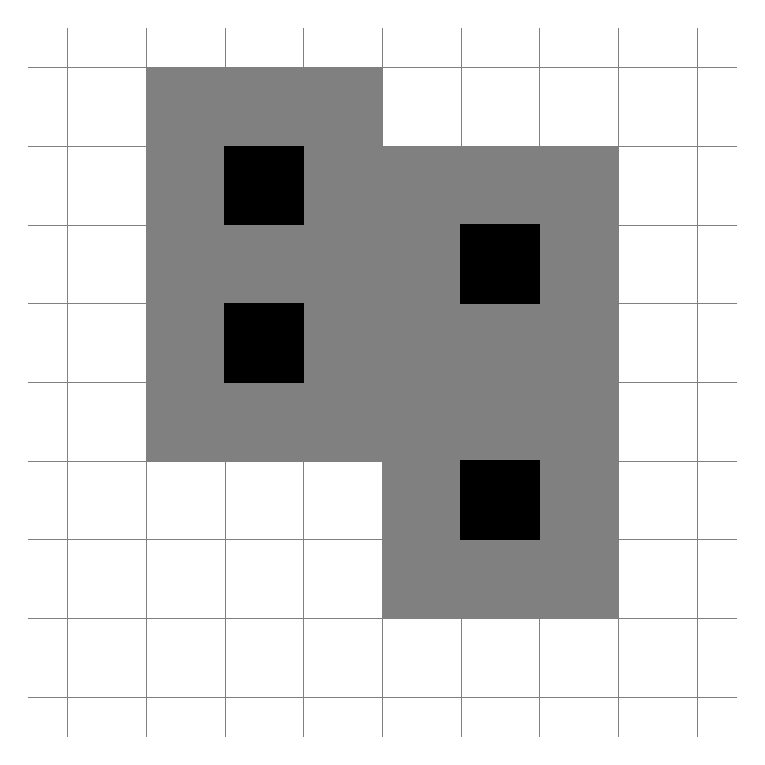
\begin{tikzpicture}
		\draw[help lines, step=1] (-4.5, -4.5) grid (4.5, 4.5);
		\foreach \x in {(-3, -1), (-3, 0), (-3, 1), (-3, 2), (-3, 3), (-2, -1), (-2, 0), (-2, 1), (-2, 2), (-2, 3), (-1, -1), (-1, 0), (-1, 1), (-1, 2), (-1, 3), (0, -3), (0, -2), (0, -1), (0, 0), (0, 1), (0, 2), (1, -3), (1, -2), (1, -1), (1, 0), (1, 1), (1, 2), (2, -3), (2, -2), (2, -1), (2, 0), (2, 1), (2, 2)}
			\filldraw[gray] \x rectangle + (1, 1);
		\foreach \x in {(-2, 0), (-2, 2), (1, 1), (1, -2)}
			\filldraw[black] \x rectangle + (1, 1);
	\end{tikzpicture}
	\caption{Binary image after binary dilation with a $3 \times 3$ pixel structuring element. The gray pixels are now set to one.}
\end{figure}

% Draw closing example after binary closing:
\begin{figure}
	\centering
	
\begin{tikzpicture}
		\draw[help lines, step=1] (-4.5, -4.5) grid (4.5, 4.5);
		\foreach \x in {(-2, 0), (-2, 1), (-2, 2), (-1, 0), (-1, 1), (0, 0), (0, 1), (1, -2), (1, -1), (1, 0), (1, 1)}
			\filldraw[gray] \x rectangle + (1, 1);
		\foreach \x in {(-2, 0), (-2, 2), (1, 1), (1, -2)}
			\filldraw[black] \x rectangle + (1, 1);
	\end{tikzpicture}
	\caption{Binary image after binary closing, i.e. dilation and erosion. Gaps have been filled.}
\end{figure}

% ------------------------------------------------------------------------

\begin{figure}
	\centering
	\begin{tikzpicture}
		\begin{axis}[
			xlabel=$x$ (-),
			ylabel=$f(x)$ (-),
			title={Measured transfer function of analogue filter},
			grid=both,
			minor grid style={gray!25},
			major grid style={gray!25},
			width=0.75\linewidth,
			no marks,
			legend pos=south east]
			\addplot[line width=1pt,solid,color=blue] table[x=x,y=y,col sep=comma]{Resources/CDF.csv};
			\draw (axis cs: 3.2554, 0) -- (axis cs: 3.2554, 0.95);
			\draw (axis cs: 0, 0.95) -- (axis cs: 3.2554, 0.95);
			\draw (axis cs: 4.2791, 0) -- (axis cs: 4.2791, 0.99);
			\draw (axis cs: 0, 0.99) -- (axis cs: 4.2791, 0.99);
			\filldraw (axis cs: 3.2554, 0.95) circle (2pt);
			\filldraw (axis cs: 4.2791, 0.99) circle (2pt);
			\addlegendentry{CDF};
		\end{axis}
	\end{tikzpicture}
	\caption{Cumulative distribution function}
\end{figure}

% ------------------------------------------------------------------------

% Draw closing example after binary dilation:
\begin{figure}
	\centering
	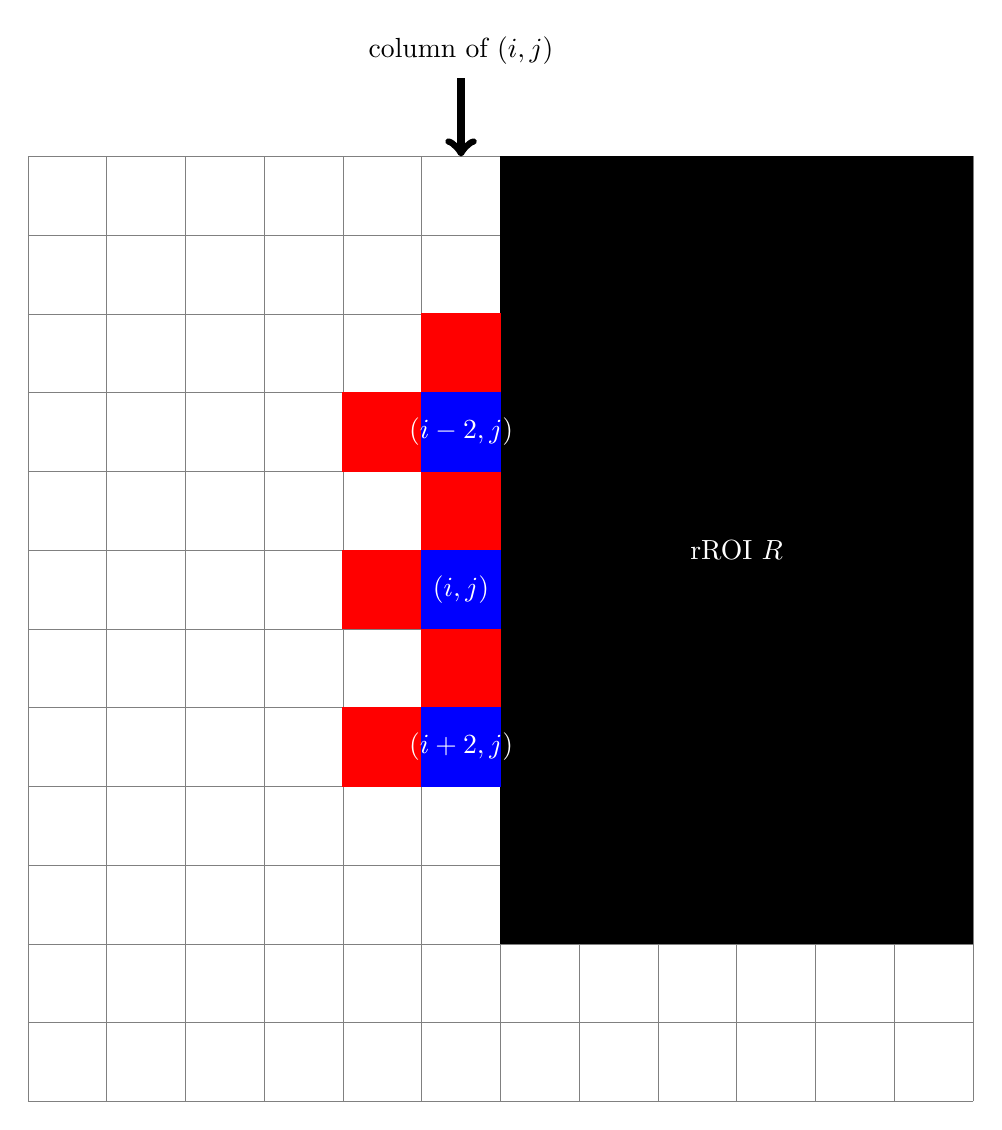
\begin{tikzpicture}
		\draw[help lines, step=1] (-6, -6) grid (6, 6);
		\foreach \i in {0, ..., 5}
			\foreach \j in {-4, ..., 5}
				\filldraw[black] (\i, \j) rectangle + (1, 1);
		\foreach \x in {(-1, 1), (-2, 0), (-1, 3), (-2, 2), ((-1, -1), (-2, -2)}
			\filldraw[red] \x rectangle + (1, 1);
		\filldraw[blue] (-1, 2) rectangle + (1, 1) node[pos=.5, color=white] {$(i - 2, j)$};
		\filldraw[blue] (-1, 0) rectangle + (1, 1) node[pos=.5, color=white] {$(i, j)$};
		\filldraw[blue] (-1, -2) rectangle + (1, 1) node[pos=.5, color=white] {$(i + 2, j)$};
		\draw[<-, line width=1mm] (-0.5, 6) -- (-0.5, 7) node[above] {column of $(i, j)$};
		\node[color=white] at (3, 1) {rROI $R$};
	\end{tikzpicture}
	\caption{The test statistics are independet for every second pixel in the column.}
\end{figure}

% ------------------------------------------------------------------------

% Set boxes to be marked for structuring element:
%markedStructuringElement = {(-1, -1), (-1, 0), (-1, 1), (0, -1), (0, 0), (0, 1), (1, -1), (1, 0), (1, 1)}

% ------------------------------------------------------------------------

% Label points:
text(-1.2, 0, '(i, j)', 'color', 'w', 'Fontsize', 10)
text(-1.4, 2, '(i - 2, j)', 'color', 'w', 'Fontsize', 10)
text(-1.4, -2, '(i + 2, j)', 'color', 'w', 'Fontsize', 10)

% title('Test statistic')

% ------------------------------------------------------------------------


\end{document}
